\documentclass[twoside]{book}

% Packages required by doxygen
\usepackage{calc}
\usepackage{doxygen}
\usepackage{graphicx}
\usepackage[utf8]{inputenc}
\usepackage{makeidx}
\usepackage{multicol}
\usepackage{multirow}
\usepackage{textcomp}
\usepackage[table]{xcolor}

% Font selection
\usepackage[T1]{fontenc}
\usepackage{mathptmx}
\usepackage[scaled=.90]{helvet}
\usepackage{courier}
\usepackage{amssymb}
\usepackage{sectsty}
\renewcommand{\familydefault}{\sfdefault}
\allsectionsfont{%
  \fontseries{bc}\selectfont%
  \color{darkgray}%
}
\renewcommand{\DoxyLabelFont}{%
  \fontseries{bc}\selectfont%
  \color{darkgray}%
}

% Page & text layout
\usepackage{geometry}
\geometry{%
  a4paper,%
  top=2.5cm,%
  bottom=2.5cm,%
  left=2.5cm,%
  right=2.5cm%
}
\tolerance=750
\hfuzz=15pt
\hbadness=750
\setlength{\emergencystretch}{15pt}
\setlength{\parindent}{0cm}
\setlength{\parskip}{0.2cm}
\makeatletter
\renewcommand{\paragraph}{%
  \@startsection{paragraph}{4}{0ex}{-1.0ex}{1.0ex}{%
    \normalfont\normalsize\bfseries\SS@parafont%
  }%
}
\renewcommand{\subparagraph}{%
  \@startsection{subparagraph}{5}{0ex}{-1.0ex}{1.0ex}{%
    \normalfont\normalsize\bfseries\SS@subparafont%
  }%
}
\makeatother

% Headers & footers
\usepackage{fancyhdr}
\pagestyle{fancyplain}
\fancyhead[LE]{\fancyplain{}{\bfseries\thepage}}
\fancyhead[CE]{\fancyplain{}{}}
\fancyhead[RE]{\fancyplain{}{\bfseries\leftmark}}
\fancyhead[LO]{\fancyplain{}{\bfseries\rightmark}}
\fancyhead[CO]{\fancyplain{}{}}
\fancyhead[RO]{\fancyplain{}{\bfseries\thepage}}
\fancyfoot[LE]{\fancyplain{}{}}
\fancyfoot[CE]{\fancyplain{}{}}
\fancyfoot[RE]{\fancyplain{}{\bfseries\scriptsize Generated on Mon Dec 7 2015 18\-:16\-:27 for Localization by Doxygen }}
\fancyfoot[LO]{\fancyplain{}{\bfseries\scriptsize Generated on Mon Dec 7 2015 18\-:16\-:27 for Localization by Doxygen }}
\fancyfoot[CO]{\fancyplain{}{}}
\fancyfoot[RO]{\fancyplain{}{}}
\renewcommand{\footrulewidth}{0.4pt}
\renewcommand{\chaptermark}[1]{%
  \markboth{#1}{}%
}
\renewcommand{\sectionmark}[1]{%
  \markright{\thesection\ #1}%
}

% Indices & bibliography
\usepackage{natbib}
\usepackage[titles]{tocloft}
\setcounter{tocdepth}{3}
\setcounter{secnumdepth}{5}
\makeindex

% Hyperlinks (required, but should be loaded last)
\usepackage{ifpdf}
\ifpdf
  \usepackage[pdftex,pagebackref=true]{hyperref}
\else
  \usepackage[ps2pdf,pagebackref=true]{hyperref}
\fi
\hypersetup{%
  colorlinks=true,%
  linkcolor=blue,%
  citecolor=blue,%
  unicode%
}

% Custom commands
\newcommand{\clearemptydoublepage}{%
  \newpage{\pagestyle{empty}\cleardoublepage}%
}


%===== C O N T E N T S =====

\begin{document}

% Titlepage & ToC
\hypersetup{pageanchor=false}
\pagenumbering{roman}
\begin{titlepage}
\vspace*{7cm}
\begin{center}%
{\Large Localization }\\
\vspace*{1cm}
{\large Generated by Doxygen 1.8.6}\\
\vspace*{0.5cm}
{\small Mon Dec 7 2015 18:16:27}\\
\end{center}
\end{titlepage}
\clearemptydoublepage
\tableofcontents
\clearemptydoublepage
\pagenumbering{arabic}
\hypersetup{pageanchor=true}

%--- Begin generated contents ---
\chapter{Bug List}
\label{bug}
\hypertarget{bug}{}

\begin{DoxyRefList}
\item[\label{bug__bug000017}%
\hypertarget{bug__bug000017}{}%
File \hyperlink{correlation__sensor__update_8h}{correlation\-\_\-sensor\-\_\-update.h} ]No known bug.  
\item[\label{bug__bug000008}%
\hypertarget{bug__bug000008}{}%
File \hyperlink{filter__parser_8h}{filter\-\_\-parser.h} ]No known bugs.  
\item[\label{bug__bug000018}%
\hypertarget{bug__bug000018}{}%
File \hyperlink{likelihood__sensor__update_8h}{likelihood\-\_\-sensor\-\_\-update.h} ]No known bug.  
\item[\label{bug__bug000001}%
\hypertarget{bug__bug000001}{}%
File \hyperlink{localization__behaviour_8h}{localization\-\_\-behaviour.h} ]No known bug.  
\item[\label{bug__bug000005}%
\hypertarget{bug__bug000005}{}%
File \hyperlink{motion__update_8h}{motion\-\_\-update.h} ]No known bug.  
\item[\label{bug__bug000009}%
\hypertarget{bug__bug000009}{}%
File \hyperlink{motion__update__parser_8h}{motion\-\_\-update\-\_\-parser.h} ]No known bugs.  
\item[\label{bug__bug000020}%
\hypertarget{bug__bug000020}{}%
File \hyperlink{occupancy__map_8h}{occupancy\-\_\-map.h} ]No known bug.  
\item[\label{bug__bug000006}%
\hypertarget{bug__bug000006}{}%
File \hyperlink{odometry__motion__update_8h}{odometry\-\_\-motion\-\_\-update.h} ]No known bug.  
\item[\label{bug__bug000021}%
\hypertarget{bug__bug000021}{}%
File \hyperlink{particle_8h}{particle.h} ]No known bug.  
\item[\label{bug__bug000002}%
\hypertarget{bug__bug000002}{}%
File \hyperlink{particle__filter_8h}{particle\-\_\-filter.h} ]No known bug.  
\item[\label{bug__bug000003}%
\hypertarget{bug__bug000003}{}%
File \hyperlink{pose__filter_8h}{pose\-\_\-filter.h} ]No known bug.  
\item[\label{bug__bug000004}%
\hypertarget{bug__bug000004}{}%
File \hyperlink{pose__filter_8hpp}{pose\-\_\-filter.hpp} ]No known bugs.  
\item[\label{bug__bug000010}%
\hypertarget{bug__bug000010}{}%
File \hyperlink{ros__parameter__parser_8h}{ros\-\_\-parameter\-\_\-parser.h} ]No known bugs  
\item[\label{bug__bug000011}%
\hypertarget{bug__bug000011}{}%
File \hyperlink{ros__topic__parser_8h}{ros\-\_\-topic\-\_\-parser.h} ]No known bugs  
\item[\label{bug__bug000014}%
\hypertarget{bug__bug000014}{}%
File \hyperlink{roulette__wheel__sampling_8h}{roulette\-\_\-wheel\-\_\-sampling.h} ]No known bug.  
\item[\label{bug__bug000015}%
\hypertarget{bug__bug000015}{}%
File \hyperlink{sampling_8h}{sampling.h} ]No known bug.  
\item[\label{bug__bug000012}%
\hypertarget{bug__bug000012}{}%
File \hyperlink{sampling__parser_8h}{sampling\-\_\-parser.h} ]No known bugs.  
\item[\label{bug__bug000019}%
\hypertarget{bug__bug000019}{}%
File \hyperlink{sensor__update_8h}{sensor\-\_\-update.h} ]No known bug.  
\item[\label{bug__bug000013}%
\hypertarget{bug__bug000013}{}%
File \hyperlink{sensor__update__parser_8h}{sensor\-\_\-update\-\_\-parser.h} ]No known bugs.  
\item[\label{bug__bug000016}%
\hypertarget{bug__bug000016}{}%
File \hyperlink{stochastic__universal__sampling_8h}{stochastic\-\_\-universal\-\_\-sampling.h} ]No known bug.  
\item[\label{bug__bug000007}%
\hypertarget{bug__bug000007}{}%
File \hyperlink{velocity__motion__update_8h}{velocity\-\_\-motion\-\_\-update.h} ]No known bug. 
\end{DoxyRefList}
\chapter{Hierarchical Index}
\section{Class Hierarchy}
This inheritance list is sorted roughly, but not completely, alphabetically\-:\begin{DoxyCompactList}
\item \contentsline{section}{Filter\-Parser}{\pageref{classFilterParser}}{}
\item \contentsline{section}{Localization\-Behaviour}{\pageref{classLocalizationBehaviour}}{}
\item \contentsline{section}{Motion\-Update}{\pageref{classMotionUpdate}}{}
\begin{DoxyCompactList}
\item \contentsline{section}{Odometry\-Motion\-Update}{\pageref{classOdometryMotionUpdate}}{}
\item \contentsline{section}{Velocity\-Motion\-Update}{\pageref{classVelocityMotionUpdate}}{}
\end{DoxyCompactList}
\item \contentsline{section}{Motion\-Update\-Parser}{\pageref{classMotionUpdateParser}}{}
\item \contentsline{section}{Occupancy\-Map}{\pageref{classOccupancyMap}}{}
\item \contentsline{section}{Particle}{\pageref{classParticle}}{}
\item \contentsline{section}{Pose\-Filter}{\pageref{classPoseFilter}}{}
\begin{DoxyCompactList}
\item \contentsline{section}{Particle\-Filter}{\pageref{classParticleFilter}}{}
\end{DoxyCompactList}
\item \contentsline{section}{Ros\-Parameter\-Parser}{\pageref{classRosParameterParser}}{}
\item \contentsline{section}{Ros\-Topic\-Parser}{\pageref{classRosTopicParser}}{}
\item \contentsline{section}{Sampling}{\pageref{classSampling}}{}
\begin{DoxyCompactList}
\item \contentsline{section}{Roulette\-Wheel\-Sampling}{\pageref{classRouletteWheelSampling}}{}
\item \contentsline{section}{Stochastic\-Universal\-Sampling}{\pageref{classStochasticUniversalSampling}}{}
\end{DoxyCompactList}
\item \contentsline{section}{Sampling\-Parser}{\pageref{classSamplingParser}}{}
\item \contentsline{section}{Sensor\-Update}{\pageref{classSensorUpdate}}{}
\begin{DoxyCompactList}
\item \contentsline{section}{Correlation\-Sensor\-Update}{\pageref{classCorrelationSensorUpdate}}{}
\item \contentsline{section}{Likelihood\-Sensor\-Update}{\pageref{classLikelihoodSensorUpdate}}{}
\end{DoxyCompactList}
\item \contentsline{section}{Sensor\-Update\-Parser}{\pageref{classSensorUpdateParser}}{}
\end{DoxyCompactList}

\chapter{Class Index}
\section{Class List}
Here are the classes, structs, unions and interfaces with brief descriptions\-:\begin{DoxyCompactList}
\item\contentsline{section}{\hyperlink{classCorrelationSensorUpdate}{Correlation\-Sensor\-Update} \\*Cross correlation model implementation of sensor update algorithm }{\pageref{classCorrelationSensorUpdate}}{}
\item\contentsline{section}{\hyperlink{classFilterParser}{Filter\-Parser} \\*Class that parses from the rosparam server the ros strategy to be used }{\pageref{classFilterParser}}{}
\item\contentsline{section}{\hyperlink{classLikelihoodSensorUpdate}{Likelihood\-Sensor\-Update} \\*Gaussian likelihood model implementation of sensor update algorithm }{\pageref{classLikelihoodSensorUpdate}}{}
\item\contentsline{section}{\hyperlink{classLocalizationBehaviour}{Localization\-Behaviour} \\*Class that sequences the pose filter algorithm from ros msgs and publishes the result }{\pageref{classLocalizationBehaviour}}{}
\item\contentsline{section}{\hyperlink{classMotionUpdate}{Motion\-Update} \\*Abstract class for implementing the motion update strategy pattern }{\pageref{classMotionUpdate}}{}
\item\contentsline{section}{\hyperlink{classMotionUpdateParser}{Motion\-Update\-Parser} \\*Class that parses from the rosparam server the motion update strategy to be used }{\pageref{classMotionUpdateParser}}{}
\item\contentsline{section}{\hyperlink{classOccupancyMap}{Occupancy\-Map} \\*Map class for creating, modifying or finding statistics from graphs }{\pageref{classOccupancyMap}}{}
\item\contentsline{section}{\hyperlink{classOdometryMotionUpdate}{Odometry\-Motion\-Update} \\*Odometry model implementation of motion update algorithm }{\pageref{classOdometryMotionUpdate}}{}
\item\contentsline{section}{\hyperlink{classParticle}{Particle} \\*Class that implements a particle for a S\-L\-A\-M algorithm }{\pageref{classParticle}}{}
\item\contentsline{section}{\hyperlink{classParticleFilter}{Particle\-Filter} \\*Implementation of the particle filter algorithm }{\pageref{classParticleFilter}}{}
\item\contentsline{section}{\hyperlink{classPoseFilter}{Pose\-Filter} \\*Abstract class for implementing the pose filter strategy pattern }{\pageref{classPoseFilter}}{}
\item\contentsline{section}{\hyperlink{classRosParameterParser}{Ros\-Parameter\-Parser} \\*Class that parses all parameters from R\-O\-S parameter server }{\pageref{classRosParameterParser}}{}
\item\contentsline{section}{\hyperlink{classRosTopicParser}{Ros\-Topic\-Parser} \\*Class that parses all topics from R\-O\-S parameter server }{\pageref{classRosTopicParser}}{}
\item\contentsline{section}{\hyperlink{classRouletteWheelSampling}{Roulette\-Wheel\-Sampling} \\*Roulette wheel implementation of sampling strategy pattern for particles }{\pageref{classRouletteWheelSampling}}{}
\item\contentsline{section}{\hyperlink{classSampling}{Sampling} \\*Abstract class for implementing the sampling strategy pattern }{\pageref{classSampling}}{}
\item\contentsline{section}{\hyperlink{classSamplingParser}{Sampling\-Parser} \\*Class that parses from the rosparam server the sampling strategy to be used }{\pageref{classSamplingParser}}{}
\item\contentsline{section}{\hyperlink{classSensorUpdate}{Sensor\-Update} \\*Abstract class for implementing the sensor update strategy pattern }{\pageref{classSensorUpdate}}{}
\item\contentsline{section}{\hyperlink{classSensorUpdateParser}{Sensor\-Update\-Parser} \\*Class that parses from the rosparam server the sensor update strategy to be used }{\pageref{classSensorUpdateParser}}{}
\item\contentsline{section}{\hyperlink{classStochasticUniversalSampling}{Stochastic\-Universal\-Sampling} \\*Stochastic universal implementation of sampling strategy pattern for particles }{\pageref{classStochasticUniversalSampling}}{}
\item\contentsline{section}{\hyperlink{classVelocityMotionUpdate}{Velocity\-Motion\-Update} \\*Velocity model implementation of motion update algorithm }{\pageref{classVelocityMotionUpdate}}{}
\end{DoxyCompactList}

\chapter{File Index}
\section{File List}
Here is a list of all documented files with brief descriptions\-:\begin{DoxyCompactList}
\item\contentsline{section}{include/localization/behaviour/\hyperlink{localization__behaviour_8h}{localization\-\_\-behaviour.\-h} }{\pageref{localization__behaviour_8h}}{}
\item\contentsline{section}{include/localization/filtering\-\_\-strategies/\hyperlink{particle__filter_8h}{particle\-\_\-filter.\-h} }{\pageref{particle__filter_8h}}{}
\item\contentsline{section}{include/localization/filtering\-\_\-strategies/\hyperlink{pose__filter_8h}{pose\-\_\-filter.\-h} }{\pageref{pose__filter_8h}}{}
\item\contentsline{section}{include/localization/filtering\-\_\-strategies/\hyperlink{pose__filter_8hpp}{pose\-\_\-filter.\-hpp} }{\pageref{pose__filter_8hpp}}{}
\item\contentsline{section}{include/localization/motion\-\_\-update\-\_\-strategies/\hyperlink{motion__update_8h}{motion\-\_\-update.\-h} }{\pageref{motion__update_8h}}{}
\item\contentsline{section}{include/localization/motion\-\_\-update\-\_\-strategies/\hyperlink{odometry__motion__update_8h}{odometry\-\_\-motion\-\_\-update.\-h} }{\pageref{odometry__motion__update_8h}}{}
\item\contentsline{section}{include/localization/motion\-\_\-update\-\_\-strategies/\hyperlink{velocity__motion__update_8h}{velocity\-\_\-motion\-\_\-update.\-h} }{\pageref{velocity__motion__update_8h}}{}
\item\contentsline{section}{include/localization/parsers/\hyperlink{filter__parser_8h}{filter\-\_\-parser.\-h} }{\pageref{filter__parser_8h}}{}
\item\contentsline{section}{include/localization/parsers/\hyperlink{motion__update__parser_8h}{motion\-\_\-update\-\_\-parser.\-h} }{\pageref{motion__update__parser_8h}}{}
\item\contentsline{section}{include/localization/parsers/\hyperlink{ros__parameter__parser_8h}{ros\-\_\-parameter\-\_\-parser.\-h} }{\pageref{ros__parameter__parser_8h}}{}
\item\contentsline{section}{include/localization/parsers/\hyperlink{ros__topic__parser_8h}{ros\-\_\-topic\-\_\-parser.\-h} }{\pageref{ros__topic__parser_8h}}{}
\item\contentsline{section}{include/localization/parsers/\hyperlink{sampling__parser_8h}{sampling\-\_\-parser.\-h} }{\pageref{sampling__parser_8h}}{}
\item\contentsline{section}{include/localization/parsers/\hyperlink{sensor__update__parser_8h}{sensor\-\_\-update\-\_\-parser.\-h} }{\pageref{sensor__update__parser_8h}}{}
\item\contentsline{section}{include/localization/sampling\-\_\-strategies/\hyperlink{roulette__wheel__sampling_8h}{roulette\-\_\-wheel\-\_\-sampling.\-h} }{\pageref{roulette__wheel__sampling_8h}}{}
\item\contentsline{section}{include/localization/sampling\-\_\-strategies/\hyperlink{sampling_8h}{sampling.\-h} }{\pageref{sampling_8h}}{}
\item\contentsline{section}{include/localization/sampling\-\_\-strategies/\hyperlink{stochastic__universal__sampling_8h}{stochastic\-\_\-universal\-\_\-sampling.\-h} }{\pageref{stochastic__universal__sampling_8h}}{}
\item\contentsline{section}{include/localization/sensor\-\_\-update\-\_\-strategies/\hyperlink{correlation__sensor__update_8h}{correlation\-\_\-sensor\-\_\-update.\-h} }{\pageref{correlation__sensor__update_8h}}{}
\item\contentsline{section}{include/localization/sensor\-\_\-update\-\_\-strategies/\hyperlink{likelihood__sensor__update_8h}{likelihood\-\_\-sensor\-\_\-update.\-h} }{\pageref{likelihood__sensor__update_8h}}{}
\item\contentsline{section}{include/localization/sensor\-\_\-update\-\_\-strategies/\hyperlink{sensor__update_8h}{sensor\-\_\-update.\-h} }{\pageref{sensor__update_8h}}{}
\item\contentsline{section}{include/localization/util/\hyperlink{occupancy__map_8h}{occupancy\-\_\-map.\-h} }{\pageref{occupancy__map_8h}}{}
\item\contentsline{section}{include/localization/util/\hyperlink{particle_8h}{particle.\-h} }{\pageref{particle_8h}}{}
\end{DoxyCompactList}

\chapter{Class Documentation}
\hypertarget{classCorrelationSensorUpdate}{\section{Correlation\-Sensor\-Update Class Reference}
\label{classCorrelationSensorUpdate}\index{Correlation\-Sensor\-Update@{Correlation\-Sensor\-Update}}
}


Cross correlation model implementation of sensor update algorithm.  




{\ttfamily \#include $<$correlation\-\_\-sensor\-\_\-update.\-h$>$}

Inheritance diagram for Correlation\-Sensor\-Update\-:\begin{figure}[H]
\begin{center}
\leavevmode
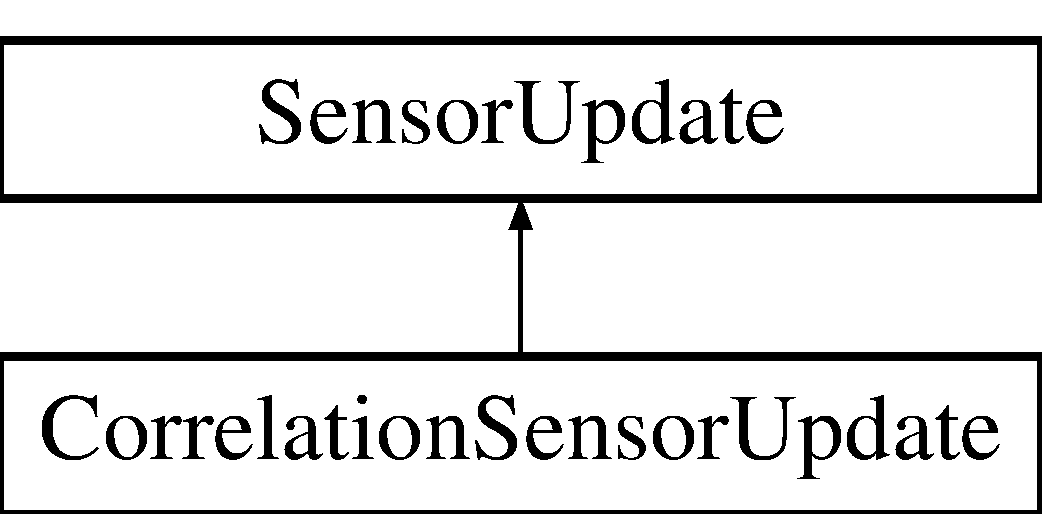
\includegraphics[height=2.000000cm]{classCorrelationSensorUpdate}
\end{center}
\end{figure}
\subsection*{Public Member Functions}
\begin{DoxyCompactItemize}
\item 
\hypertarget{classCorrelationSensorUpdate_a0f43ac21ac425802edb523f5f065a0b0}{\hyperlink{classCorrelationSensorUpdate_a0f43ac21ac425802edb523f5f065a0b0}{Correlation\-Sensor\-Update} ()}\label{classCorrelationSensorUpdate_a0f43ac21ac425802edb523f5f065a0b0}

\begin{DoxyCompactList}\small\item\em Default Constructor. \end{DoxyCompactList}\item 
double \hyperlink{classCorrelationSensorUpdate_a72b2bd8daa21b7c76de0eb306e579906}{a\-\_\-posteriori} (double a\-\_\-priori, \hyperlink{occupancy__map_8h_aea86d1b633e7d9b44b660a39fa9b50f7}{Occupancy\-Map\-Ptr} a\-\_\-priori\-\_\-map, geometry\-\_\-msgs\-::\-Pose\-With\-Covariance\-Stamped pose, const sensor\-\_\-msgs\-::\-Laser\-Scan\-::\-Const\-Ptr \&msg)
\end{DoxyCompactItemize}
\subsection*{Additional Inherited Members}


\subsection{Detailed Description}
Cross correlation model implementation of sensor update algorithm. 

\subsection{Member Function Documentation}
\hypertarget{classCorrelationSensorUpdate_a72b2bd8daa21b7c76de0eb306e579906}{\index{Correlation\-Sensor\-Update@{Correlation\-Sensor\-Update}!a\-\_\-posteriori@{a\-\_\-posteriori}}
\index{a\-\_\-posteriori@{a\-\_\-posteriori}!CorrelationSensorUpdate@{Correlation\-Sensor\-Update}}
\subsubsection[{a\-\_\-posteriori}]{\setlength{\rightskip}{0pt plus 5cm}double Correlation\-Sensor\-Update\-::a\-\_\-posteriori (
\begin{DoxyParamCaption}
\item[{double}]{a\-\_\-priori, }
\item[{{\bf Occupancy\-Map\-Ptr}}]{a\-\_\-priori\-\_\-map, }
\item[{geometry\-\_\-msgs\-::\-Pose\-With\-Covariance\-Stamped}]{pose, }
\item[{const sensor\-\_\-msgs\-::\-Laser\-Scan\-::\-Const\-Ptr \&}]{msg}
\end{DoxyParamCaption}
)\hspace{0.3cm}{\ttfamily [virtual]}}}\label{classCorrelationSensorUpdate_a72b2bd8daa21b7c76de0eb306e579906}
Get a posteriori probability of being in a pose given the msg. 
\begin{DoxyParams}{Parameters}
{\em a\-\_\-priori} & a priori probability of being in a pose. \\
\hline
{\em a\-\_\-priori\-\_\-map} & a priori pointer to believed map. \\
\hline
{\em pose} & believed pose. \\
\hline
{\em msg} & recieved scan msg. \\
\hline
\end{DoxyParams}
\begin{DoxyReturn}{Returns}
a posteriori probability 
\end{DoxyReturn}


Implements \hyperlink{classSensorUpdate_a9bd0792d09b9425b854c6220b6712a52}{Sensor\-Update}.



The documentation for this class was generated from the following file\-:\begin{DoxyCompactItemize}
\item 
include/localization/sensor\-\_\-update\-\_\-strategies/\hyperlink{correlation__sensor__update_8h}{correlation\-\_\-sensor\-\_\-update.\-h}\end{DoxyCompactItemize}

\hypertarget{classFilterParser}{\section{Filter\-Parser Class Reference}
\label{classFilterParser}\index{Filter\-Parser@{Filter\-Parser}}
}


Class that parses from the rosparam server the ros strategy to be used.  




{\ttfamily \#include $<$filter\-\_\-parser.\-h$>$}

\subsection*{Public Member Functions}
\begin{DoxyCompactItemize}
\item 
\hypertarget{classFilterParser_a9dacc645f2fb48cdd505e707c712150b}{\hyperlink{classFilterParser_a9dacc645f2fb48cdd505e707c712150b}{Filter\-Parser} (ros\-::\-Node\-Handle nh)}\label{classFilterParser_a9dacc645f2fb48cdd505e707c712150b}

\begin{DoxyCompactList}\small\item\em Default Constructor. \end{DoxyCompactList}\item 
\hypertarget{classFilterParser_a5444670243e803404cd51a9863322ac9}{\hyperlink{classFilterParser_a5444670243e803404cd51a9863322ac9}{$\sim$\-Filter\-Parser} ()}\label{classFilterParser_a5444670243e803404cd51a9863322ac9}

\begin{DoxyCompactList}\small\item\em Class Deconstructor. \end{DoxyCompactList}\item 
\hypertarget{classFilterParser_af815f5bbda50c90b5d741ceec57372a0}{\hyperlink{pose__filter_8h_a9df59d7c2f322f00bdd8eccab6d3fd73}{Pose\-Filter\-Ptr} \hyperlink{classFilterParser_af815f5bbda50c90b5d741ceec57372a0}{get\-\_\-filter} ()}\label{classFilterParser_af815f5bbda50c90b5d741ceec57372a0}

\begin{DoxyCompactList}\small\item\em Get parsed filter strategy implementation. \end{DoxyCompactList}\end{DoxyCompactItemize}


\subsection{Detailed Description}
Class that parses from the rosparam server the ros strategy to be used. 

The documentation for this class was generated from the following file\-:\begin{DoxyCompactItemize}
\item 
include/localization/parsers/\hyperlink{filter__parser_8h}{filter\-\_\-parser.\-h}\end{DoxyCompactItemize}

\hypertarget{classLikelihoodSensorUpdate}{\section{Likelihood\-Sensor\-Update Class Reference}
\label{classLikelihoodSensorUpdate}\index{Likelihood\-Sensor\-Update@{Likelihood\-Sensor\-Update}}
}


Gaussian likelihood model implementation of sensor update algorithm.  




{\ttfamily \#include $<$likelihood\-\_\-sensor\-\_\-update.\-h$>$}

Inheritance diagram for Likelihood\-Sensor\-Update\-:\begin{figure}[H]
\begin{center}
\leavevmode
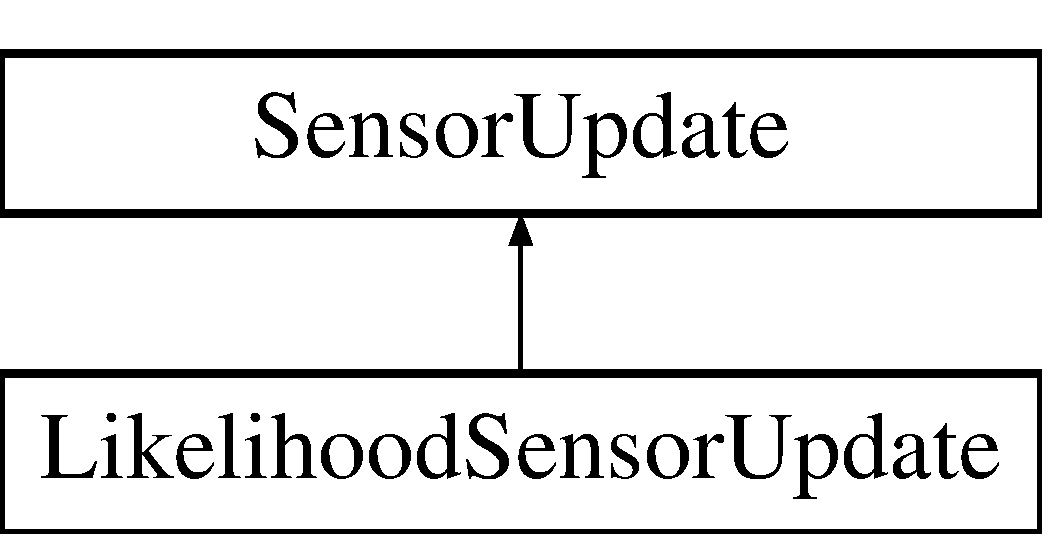
\includegraphics[height=2.000000cm]{classLikelihoodSensorUpdate}
\end{center}
\end{figure}
\subsection*{Public Member Functions}
\begin{DoxyCompactItemize}
\item 
\hypertarget{classLikelihoodSensorUpdate_a60424de72efee82d70d13061dcb65ae2}{\hyperlink{classLikelihoodSensorUpdate_a60424de72efee82d70d13061dcb65ae2}{Likelihood\-Sensor\-Update} ()}\label{classLikelihoodSensorUpdate_a60424de72efee82d70d13061dcb65ae2}

\begin{DoxyCompactList}\small\item\em Default Constructor. \end{DoxyCompactList}\item 
\hyperlink{classLikelihoodSensorUpdate_a342698e21192ccbab6cfbdec8fae0e46}{Likelihood\-Sensor\-Update} (double z\-\_\-rand, double z\-\_\-var)
\item 
double \hyperlink{classLikelihoodSensorUpdate_aa7a4eaae56fb86af98f428b598f46962}{a\-\_\-posteriori} (double a\-\_\-priori, \hyperlink{occupancy__map_8h_aea86d1b633e7d9b44b660a39fa9b50f7}{Occupancy\-Map\-Ptr} a\-\_\-priori\-\_\-map, geometry\-\_\-msgs\-::\-Pose\-With\-Covariance\-Stamped pose, const sensor\-\_\-msgs\-::\-Laser\-Scan\-::\-Const\-Ptr \&msg)
\end{DoxyCompactItemize}
\subsection*{Additional Inherited Members}


\subsection{Detailed Description}
Gaussian likelihood model implementation of sensor update algorithm. 

\subsection{Constructor \& Destructor Documentation}
\hypertarget{classLikelihoodSensorUpdate_a342698e21192ccbab6cfbdec8fae0e46}{\index{Likelihood\-Sensor\-Update@{Likelihood\-Sensor\-Update}!Likelihood\-Sensor\-Update@{Likelihood\-Sensor\-Update}}
\index{Likelihood\-Sensor\-Update@{Likelihood\-Sensor\-Update}!LikelihoodSensorUpdate@{Likelihood\-Sensor\-Update}}
\subsubsection[{Likelihood\-Sensor\-Update}]{\setlength{\rightskip}{0pt plus 5cm}Likelihood\-Sensor\-Update\-::\-Likelihood\-Sensor\-Update (
\begin{DoxyParamCaption}
\item[{double}]{z\-\_\-rand, }
\item[{double}]{z\-\_\-var}
\end{DoxyParamCaption}
)}}\label{classLikelihoodSensorUpdate_a342698e21192ccbab6cfbdec8fae0e46}
Class constructor 
\begin{DoxyParams}{Parameters}
{\em z\-\_\-rand} & measurement bias. \\
\hline
{\em z\-\_\-var} & measurement variance . \\
\hline
\end{DoxyParams}


\subsection{Member Function Documentation}
\hypertarget{classLikelihoodSensorUpdate_aa7a4eaae56fb86af98f428b598f46962}{\index{Likelihood\-Sensor\-Update@{Likelihood\-Sensor\-Update}!a\-\_\-posteriori@{a\-\_\-posteriori}}
\index{a\-\_\-posteriori@{a\-\_\-posteriori}!LikelihoodSensorUpdate@{Likelihood\-Sensor\-Update}}
\subsubsection[{a\-\_\-posteriori}]{\setlength{\rightskip}{0pt plus 5cm}double Likelihood\-Sensor\-Update\-::a\-\_\-posteriori (
\begin{DoxyParamCaption}
\item[{double}]{a\-\_\-priori, }
\item[{{\bf Occupancy\-Map\-Ptr}}]{a\-\_\-priori\-\_\-map, }
\item[{geometry\-\_\-msgs\-::\-Pose\-With\-Covariance\-Stamped}]{pose, }
\item[{const sensor\-\_\-msgs\-::\-Laser\-Scan\-::\-Const\-Ptr \&}]{msg}
\end{DoxyParamCaption}
)\hspace{0.3cm}{\ttfamily [virtual]}}}\label{classLikelihoodSensorUpdate_aa7a4eaae56fb86af98f428b598f46962}
Get a posteriori probability of being in a pose given the msg. 
\begin{DoxyParams}{Parameters}
{\em a\-\_\-priori} & a priori probability of being in a pose. \\
\hline
{\em a\-\_\-priori\-\_\-map} & a priori pointer to believed map. \\
\hline
{\em pose} & believed pose. \\
\hline
{\em msg} & recieved scan msg. \\
\hline
\end{DoxyParams}
\begin{DoxyReturn}{Returns}
a posteriori probability 
\end{DoxyReturn}


Implements \hyperlink{classSensorUpdate_a9bd0792d09b9425b854c6220b6712a52}{Sensor\-Update}.



The documentation for this class was generated from the following file\-:\begin{DoxyCompactItemize}
\item 
include/localization/sensor\-\_\-update\-\_\-strategies/\hyperlink{likelihood__sensor__update_8h}{likelihood\-\_\-sensor\-\_\-update.\-h}\end{DoxyCompactItemize}

\hypertarget{classLocalizationBehaviour}{\section{Localization\-Behaviour Class Reference}
\label{classLocalizationBehaviour}\index{Localization\-Behaviour@{Localization\-Behaviour}}
}


Class that sequences the pose filter algorithm from ros msgs and publishes the result.  




{\ttfamily \#include $<$localization\-\_\-behaviour.\-h$>$}

\subsection*{Public Member Functions}
\begin{DoxyCompactItemize}
\item 
\hypertarget{classLocalizationBehaviour_a8fbdf12412fc69f2eed036a3d003c808}{\hyperlink{classLocalizationBehaviour_a8fbdf12412fc69f2eed036a3d003c808}{Localization\-Behaviour} ()}\label{classLocalizationBehaviour_a8fbdf12412fc69f2eed036a3d003c808}

\begin{DoxyCompactList}\small\item\em Default Constructor. \end{DoxyCompactList}\item 
\hyperlink{classLocalizationBehaviour_a4214dad5f0576a7d4d386476c35a00cc}{Localization\-Behaviour} (\hyperlink{pose__filter_8h_a9df59d7c2f322f00bdd8eccab6d3fd73}{Pose\-Filter\-Ptr} filter)
\item 
void \hyperlink{classLocalizationBehaviour_a3f7e87ea9de49757cf61624d3cb38289}{set\-\_\-filter} (\hyperlink{pose__filter_8h_a9df59d7c2f322f00bdd8eccab6d3fd73}{Pose\-Filter\-Ptr} filter)
\item 
void \hyperlink{classLocalizationBehaviour_a71f26956851efb42ec0d41f67d5fb744}{map\-\_\-callback} (const nav\-\_\-msgs\-::\-Occupancy\-Grid\-::\-Const\-Ptr \&msg)
\item 
void \hyperlink{classLocalizationBehaviour_a6d66815f5aaf22643a4b6ddc2a406f7d}{odometry\-\_\-callback} (const nav\-\_\-msgs\-::\-Odometry\-::\-Const\-Ptr \&msg)
\item 
void \hyperlink{classLocalizationBehaviour_aca2be6938ff49e7c2d6701fabe8612f3}{laserscan\-\_\-callback} (const sensor\-\_\-msgs\-::\-Laser\-Scan\-::\-Const\-Ptr \&msg)
\item 
void \hyperlink{classLocalizationBehaviour_aeba3e969c5065fbdaa8358b697a125d8}{publish\-\_\-array} (std\-::vector$<$ geometry\-\_\-msgs\-::\-Pose\-With\-Covariance\-Stamped $>$ arrays, std\-\_\-msgs\-::\-Header header)
\item 
void \hyperlink{classLocalizationBehaviour_aef0b0f4bd1c23b8dd7ce8bb544b2a9d8}{publish\-\_\-estimated\-\_\-tf} (geometry\-\_\-msgs\-::\-Pose\-With\-Covariance\-Stamped pose, std\-\_\-msgs\-::\-Header header)
\item 
void \hyperlink{classLocalizationBehaviour_ac6180e3b8ac4fc8497d92d99acb8726f}{set\-\_\-array\-\_\-publisher} (ros\-::\-Publisher pose\-\_\-array\-\_\-pub)
\end{DoxyCompactItemize}


\subsection{Detailed Description}
Class that sequences the pose filter algorithm from ros msgs and publishes the result. 

\subsection{Constructor \& Destructor Documentation}
\hypertarget{classLocalizationBehaviour_a4214dad5f0576a7d4d386476c35a00cc}{\index{Localization\-Behaviour@{Localization\-Behaviour}!Localization\-Behaviour@{Localization\-Behaviour}}
\index{Localization\-Behaviour@{Localization\-Behaviour}!LocalizationBehaviour@{Localization\-Behaviour}}
\subsubsection[{Localization\-Behaviour}]{\setlength{\rightskip}{0pt plus 5cm}Localization\-Behaviour\-::\-Localization\-Behaviour (
\begin{DoxyParamCaption}
\item[{{\bf Pose\-Filter\-Ptr}}]{filter}
\end{DoxyParamCaption}
)}}\label{classLocalizationBehaviour_a4214dad5f0576a7d4d386476c35a00cc}
Class constructor from pose filter 
\begin{DoxyParams}{Parameters}
{\em filter} & filter implementation \\
\hline
\end{DoxyParams}


\subsection{Member Function Documentation}
\hypertarget{classLocalizationBehaviour_aca2be6938ff49e7c2d6701fabe8612f3}{\index{Localization\-Behaviour@{Localization\-Behaviour}!laserscan\-\_\-callback@{laserscan\-\_\-callback}}
\index{laserscan\-\_\-callback@{laserscan\-\_\-callback}!LocalizationBehaviour@{Localization\-Behaviour}}
\subsubsection[{laserscan\-\_\-callback}]{\setlength{\rightskip}{0pt plus 5cm}void Localization\-Behaviour\-::laserscan\-\_\-callback (
\begin{DoxyParamCaption}
\item[{const sensor\-\_\-msgs\-::\-Laser\-Scan\-::\-Const\-Ptr \&}]{msg}
\end{DoxyParamCaption}
)}}\label{classLocalizationBehaviour_aca2be6938ff49e7c2d6701fabe8612f3}
Callback method when the laser msg is recieved. The sensor update is called from within. 
\begin{DoxyParams}{Parameters}
{\em msg} & sensor msg pointer. \\
\hline
\end{DoxyParams}
\hypertarget{classLocalizationBehaviour_a71f26956851efb42ec0d41f67d5fb744}{\index{Localization\-Behaviour@{Localization\-Behaviour}!map\-\_\-callback@{map\-\_\-callback}}
\index{map\-\_\-callback@{map\-\_\-callback}!LocalizationBehaviour@{Localization\-Behaviour}}
\subsubsection[{map\-\_\-callback}]{\setlength{\rightskip}{0pt plus 5cm}void Localization\-Behaviour\-::map\-\_\-callback (
\begin{DoxyParamCaption}
\item[{const nav\-\_\-msgs\-::\-Occupancy\-Grid\-::\-Const\-Ptr \&}]{msg}
\end{DoxyParamCaption}
)}}\label{classLocalizationBehaviour_a71f26956851efb42ec0d41f67d5fb744}
Callback method when the map is recieved or updated. 
\begin{DoxyParams}{Parameters}
{\em msg} & map msg pointer. \\
\hline
\end{DoxyParams}
\hypertarget{classLocalizationBehaviour_a6d66815f5aaf22643a4b6ddc2a406f7d}{\index{Localization\-Behaviour@{Localization\-Behaviour}!odometry\-\_\-callback@{odometry\-\_\-callback}}
\index{odometry\-\_\-callback@{odometry\-\_\-callback}!LocalizationBehaviour@{Localization\-Behaviour}}
\subsubsection[{odometry\-\_\-callback}]{\setlength{\rightskip}{0pt plus 5cm}void Localization\-Behaviour\-::odometry\-\_\-callback (
\begin{DoxyParamCaption}
\item[{const nav\-\_\-msgs\-::\-Odometry\-::\-Const\-Ptr \&}]{msg}
\end{DoxyParamCaption}
)}}\label{classLocalizationBehaviour_a6d66815f5aaf22643a4b6ddc2a406f7d}
Callback method when the odometry msg is recieved. The motion update is called from within. 
\begin{DoxyParams}{Parameters}
{\em msg} & odometry msg pointer. \\
\hline
\end{DoxyParams}
\hypertarget{classLocalizationBehaviour_aeba3e969c5065fbdaa8358b697a125d8}{\index{Localization\-Behaviour@{Localization\-Behaviour}!publish\-\_\-array@{publish\-\_\-array}}
\index{publish\-\_\-array@{publish\-\_\-array}!LocalizationBehaviour@{Localization\-Behaviour}}
\subsubsection[{publish\-\_\-array}]{\setlength{\rightskip}{0pt plus 5cm}void Localization\-Behaviour\-::publish\-\_\-array (
\begin{DoxyParamCaption}
\item[{std\-::vector$<$ geometry\-\_\-msgs\-::\-Pose\-With\-Covariance\-Stamped $>$}]{arrays, }
\item[{std\-\_\-msgs\-::\-Header}]{header}
\end{DoxyParamCaption}
)}}\label{classLocalizationBehaviour_aeba3e969c5065fbdaa8358b697a125d8}
Publish an array of poses. 
\begin{DoxyParams}{Parameters}
{\em arrays} & Array of poses to publish. \\
\hline
{\em header} & Header with time and frame id of the arrays. \\
\hline
\end{DoxyParams}
\hypertarget{classLocalizationBehaviour_aef0b0f4bd1c23b8dd7ce8bb544b2a9d8}{\index{Localization\-Behaviour@{Localization\-Behaviour}!publish\-\_\-estimated\-\_\-tf@{publish\-\_\-estimated\-\_\-tf}}
\index{publish\-\_\-estimated\-\_\-tf@{publish\-\_\-estimated\-\_\-tf}!LocalizationBehaviour@{Localization\-Behaviour}}
\subsubsection[{publish\-\_\-estimated\-\_\-tf}]{\setlength{\rightskip}{0pt plus 5cm}void Localization\-Behaviour\-::publish\-\_\-estimated\-\_\-tf (
\begin{DoxyParamCaption}
\item[{geometry\-\_\-msgs\-::\-Pose\-With\-Covariance\-Stamped}]{pose, }
\item[{std\-\_\-msgs\-::\-Header}]{header}
\end{DoxyParamCaption}
)}}\label{classLocalizationBehaviour_aef0b0f4bd1c23b8dd7ce8bb544b2a9d8}
Publish a tf between the map and the estimated pose. 
\begin{DoxyParams}{Parameters}
{\em pose} & estimated pose. \\
\hline
{\em header} & Header with time and frame id of the pose. \\
\hline
\end{DoxyParams}
\hypertarget{classLocalizationBehaviour_ac6180e3b8ac4fc8497d92d99acb8726f}{\index{Localization\-Behaviour@{Localization\-Behaviour}!set\-\_\-array\-\_\-publisher@{set\-\_\-array\-\_\-publisher}}
\index{set\-\_\-array\-\_\-publisher@{set\-\_\-array\-\_\-publisher}!LocalizationBehaviour@{Localization\-Behaviour}}
\subsubsection[{set\-\_\-array\-\_\-publisher}]{\setlength{\rightskip}{0pt plus 5cm}void Localization\-Behaviour\-::set\-\_\-array\-\_\-publisher (
\begin{DoxyParamCaption}
\item[{ros\-::\-Publisher}]{pose\-\_\-array\-\_\-pub}
\end{DoxyParamCaption}
)}}\label{classLocalizationBehaviour_ac6180e3b8ac4fc8497d92d99acb8726f}
Setter of the array publisher. 
\begin{DoxyParams}{Parameters}
{\em pose\-\_\-array\-\_\-pub} & \\
\hline
\end{DoxyParams}
\hypertarget{classLocalizationBehaviour_a3f7e87ea9de49757cf61624d3cb38289}{\index{Localization\-Behaviour@{Localization\-Behaviour}!set\-\_\-filter@{set\-\_\-filter}}
\index{set\-\_\-filter@{set\-\_\-filter}!LocalizationBehaviour@{Localization\-Behaviour}}
\subsubsection[{set\-\_\-filter}]{\setlength{\rightskip}{0pt plus 5cm}void Localization\-Behaviour\-::set\-\_\-filter (
\begin{DoxyParamCaption}
\item[{{\bf Pose\-Filter\-Ptr}}]{filter}
\end{DoxyParamCaption}
)}}\label{classLocalizationBehaviour_a3f7e87ea9de49757cf61624d3cb38289}
Set the filter implementation 
\begin{DoxyParams}{Parameters}
{\em filter} & pose filter implementation. \\
\hline
\end{DoxyParams}


The documentation for this class was generated from the following file\-:\begin{DoxyCompactItemize}
\item 
include/localization/behaviour/\hyperlink{localization__behaviour_8h}{localization\-\_\-behaviour.\-h}\end{DoxyCompactItemize}

\hypertarget{classMotionUpdate}{\section{Motion\-Update Class Reference}
\label{classMotionUpdate}\index{Motion\-Update@{Motion\-Update}}
}


Abstract class for implementing the motion update strategy pattern.  




{\ttfamily \#include $<$motion\-\_\-update.\-h$>$}

Inheritance diagram for Motion\-Update\-:\begin{figure}[H]
\begin{center}
\leavevmode
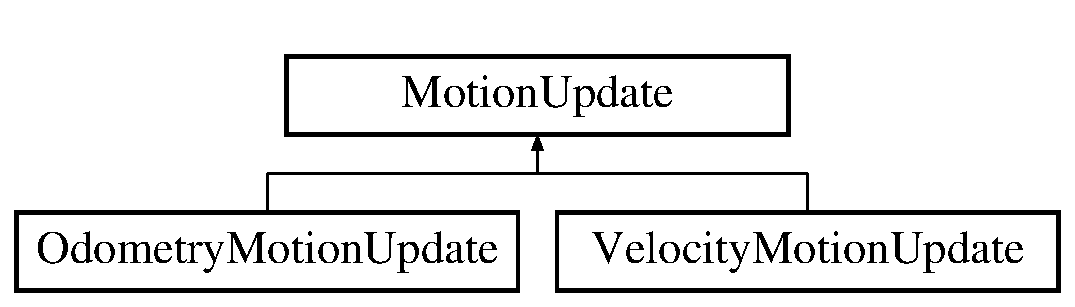
\includegraphics[height=2.000000cm]{classMotionUpdate}
\end{center}
\end{figure}
\subsection*{Public Member Functions}
\begin{DoxyCompactItemize}
\item 
virtual \\*
geometry\-\_\-msgs\-::\-Pose\-With\-Covariance\-Stamped \hyperlink{classMotionUpdate_a86e028d43981218ddf6e354e8f201e75}{predict} (geometry\-\_\-msgs\-::\-Pose\-With\-Covariance\-Stamped pose, const nav\-\_\-msgs\-::\-Odometry\-::\-Const\-Ptr \&old\-\_\-msg, const nav\-\_\-msgs\-::\-Odometry\-::\-Const\-Ptr \&new\-\_\-msg)=0
\begin{DoxyCompactList}\small\item\em Virtual Deconstructor. \end{DoxyCompactList}\item 
std\-::string \hyperlink{classMotionUpdate_aaf0a65c8acbc92f8f199e874f596db13}{get\-\_\-name} ()
\item 
void \hyperlink{classMotionUpdate_a26584d87c8360faedc8522bd163da49b}{set\-\_\-variance} (std\-::vector$<$ double $>$ variance)
\end{DoxyCompactItemize}
\subsection*{Protected Attributes}
\begin{DoxyCompactItemize}
\item 
\hypertarget{classMotionUpdate_abbc6aa3b84948633b9f78457a8b8c350}{std\-::string \hyperlink{classMotionUpdate_abbc6aa3b84948633b9f78457a8b8c350}{\-\_\-name}}\label{classMotionUpdate_abbc6aa3b84948633b9f78457a8b8c350}

\begin{DoxyCompactList}\small\item\em algorithm name. \end{DoxyCompactList}\item 
\hypertarget{classMotionUpdate_afd6ec5a2d192392fd23a0d637cce71be}{std\-::vector$<$ double $>$ \hyperlink{classMotionUpdate_afd6ec5a2d192392fd23a0d637cce71be}{\-\_\-variance}}\label{classMotionUpdate_afd6ec5a2d192392fd23a0d637cce71be}

\begin{DoxyCompactList}\small\item\em prediction variance. \end{DoxyCompactList}\item 
\hypertarget{classMotionUpdate_aad51f40e81e60f672035f0a43bb352ad}{std\-::random\-\_\-device \hyperlink{classMotionUpdate_aad51f40e81e60f672035f0a43bb352ad}{rd}}\label{classMotionUpdate_aad51f40e81e60f672035f0a43bb352ad}

\begin{DoxyCompactList}\small\item\em random device \end{DoxyCompactList}\item 
\hypertarget{classMotionUpdate_ae69a23e3978d216c73c296984eb82ad0}{std\-::mt19937 \hyperlink{classMotionUpdate_ae69a23e3978d216c73c296984eb82ad0}{\-\_\-gen}}\label{classMotionUpdate_ae69a23e3978d216c73c296984eb82ad0}

\begin{DoxyCompactList}\small\item\em random generator. \end{DoxyCompactList}\end{DoxyCompactItemize}


\subsection{Detailed Description}
Abstract class for implementing the motion update strategy pattern. 

\subsection{Member Function Documentation}
\hypertarget{classMotionUpdate_aaf0a65c8acbc92f8f199e874f596db13}{\index{Motion\-Update@{Motion\-Update}!get\-\_\-name@{get\-\_\-name}}
\index{get\-\_\-name@{get\-\_\-name}!MotionUpdate@{Motion\-Update}}
\subsubsection[{get\-\_\-name}]{\setlength{\rightskip}{0pt plus 5cm}std\-::string Motion\-Update\-::get\-\_\-name (
\begin{DoxyParamCaption}
{}
\end{DoxyParamCaption}
)}}\label{classMotionUpdate_aaf0a65c8acbc92f8f199e874f596db13}
Get algorithm's name \begin{DoxyReturn}{Returns}

\end{DoxyReturn}
\hypertarget{classMotionUpdate_a86e028d43981218ddf6e354e8f201e75}{\index{Motion\-Update@{Motion\-Update}!predict@{predict}}
\index{predict@{predict}!MotionUpdate@{Motion\-Update}}
\subsubsection[{predict}]{\setlength{\rightskip}{0pt plus 5cm}virtual geometry\-\_\-msgs\-::\-Pose\-With\-Covariance\-Stamped Motion\-Update\-::predict (
\begin{DoxyParamCaption}
\item[{geometry\-\_\-msgs\-::\-Pose\-With\-Covariance\-Stamped}]{pose, }
\item[{const nav\-\_\-msgs\-::\-Odometry\-::\-Const\-Ptr \&}]{old\-\_\-msg, }
\item[{const nav\-\_\-msgs\-::\-Odometry\-::\-Const\-Ptr \&}]{new\-\_\-msg}
\end{DoxyParamCaption}
)\hspace{0.3cm}{\ttfamily [pure virtual]}}}\label{classMotionUpdate_a86e028d43981218ddf6e354e8f201e75}


Virtual Deconstructor. 

Predict the new pose. 
\begin{DoxyParams}{Parameters}
{\em pose} & current pose. \\
\hline
{\em old\-\_\-msg} & last odometry msg. \\
\hline
{\em new\-\_\-msg} & new odometry msg. \\
\hline
\end{DoxyParams}
\begin{DoxyReturn}{Returns}

\end{DoxyReturn}


Implemented in \hyperlink{classOdometryMotionUpdate_aae9430006166324a62f4f7fbbd510841}{Odometry\-Motion\-Update}, and \hyperlink{classVelocityMotionUpdate_a1b532d900fd3393e70f7a70f153c3e08}{Velocity\-Motion\-Update}.

\hypertarget{classMotionUpdate_a26584d87c8360faedc8522bd163da49b}{\index{Motion\-Update@{Motion\-Update}!set\-\_\-variance@{set\-\_\-variance}}
\index{set\-\_\-variance@{set\-\_\-variance}!MotionUpdate@{Motion\-Update}}
\subsubsection[{set\-\_\-variance}]{\setlength{\rightskip}{0pt plus 5cm}void Motion\-Update\-::set\-\_\-variance (
\begin{DoxyParamCaption}
\item[{std\-::vector$<$ double $>$}]{variance}
\end{DoxyParamCaption}
)}}\label{classMotionUpdate_a26584d87c8360faedc8522bd163da49b}
Set prediction variance. 
\begin{DoxyParams}{Parameters}
{\em variance} & \\
\hline
\end{DoxyParams}


The documentation for this class was generated from the following file\-:\begin{DoxyCompactItemize}
\item 
include/localization/motion\-\_\-update\-\_\-strategies/\hyperlink{motion__update_8h}{motion\-\_\-update.\-h}\end{DoxyCompactItemize}

\hypertarget{classMotionUpdateParser}{\section{Motion\-Update\-Parser Class Reference}
\label{classMotionUpdateParser}\index{Motion\-Update\-Parser@{Motion\-Update\-Parser}}
}


Class that parses from the rosparam server the motion update strategy to be used.  




{\ttfamily \#include $<$motion\-\_\-update\-\_\-parser.\-h$>$}

\subsection*{Public Member Functions}
\begin{DoxyCompactItemize}
\item 
\hypertarget{classMotionUpdateParser_a497ae86be65c8c0e74fc1c7a6aa2f307}{\hyperlink{classMotionUpdateParser_a497ae86be65c8c0e74fc1c7a6aa2f307}{Motion\-Update\-Parser} (ros\-::\-Node\-Handle nh)}\label{classMotionUpdateParser_a497ae86be65c8c0e74fc1c7a6aa2f307}

\begin{DoxyCompactList}\small\item\em Default Constructor. \end{DoxyCompactList}\item 
\hypertarget{classMotionUpdateParser_a55e34b2f151f2d26565a36a7e8c216f7}{\hyperlink{classMotionUpdateParser_a55e34b2f151f2d26565a36a7e8c216f7}{$\sim$\-Motion\-Update\-Parser} ()}\label{classMotionUpdateParser_a55e34b2f151f2d26565a36a7e8c216f7}

\begin{DoxyCompactList}\small\item\em Class Deconstructor. \end{DoxyCompactList}\item 
\hypertarget{classMotionUpdateParser_a6cbea57e2617ccfaf523f3c04fbf7cf0}{\hyperlink{motion__update_8h_aec1cf0d54c70c4dacac639ab488bf948}{Motion\-Update\-Ptr} \hyperlink{classMotionUpdateParser_a6cbea57e2617ccfaf523f3c04fbf7cf0}{get\-\_\-motion\-\_\-update} ()}\label{classMotionUpdateParser_a6cbea57e2617ccfaf523f3c04fbf7cf0}

\begin{DoxyCompactList}\small\item\em Get parsed motion update strategy implementation. \end{DoxyCompactList}\end{DoxyCompactItemize}


\subsection{Detailed Description}
Class that parses from the rosparam server the motion update strategy to be used. 

The documentation for this class was generated from the following file\-:\begin{DoxyCompactItemize}
\item 
include/localization/parsers/\hyperlink{motion__update__parser_8h}{motion\-\_\-update\-\_\-parser.\-h}\end{DoxyCompactItemize}

\hypertarget{classOccupancyMap}{\section{Occupancy\-Map Class Reference}
\label{classOccupancyMap}\index{Occupancy\-Map@{Occupancy\-Map}}
}


Map class for creating, modifying or finding statistics from graphs.  




{\ttfamily \#include $<$occupancy\-\_\-map.\-h$>$}

\subsection*{Public Member Functions}
\begin{DoxyCompactItemize}
\item 
\hypertarget{classOccupancyMap_ada3a7ee4c7039ae8a8eeb6f8b59df2a9}{\hyperlink{classOccupancyMap_ada3a7ee4c7039ae8a8eeb6f8b59df2a9}{Occupancy\-Map} ()}\label{classOccupancyMap_ada3a7ee4c7039ae8a8eeb6f8b59df2a9}

\begin{DoxyCompactList}\small\item\em Default Constructor. \end{DoxyCompactList}\item 
\hyperlink{classOccupancyMap_a29d5ee8d5c52daf99c9295e0e1a93233}{Occupancy\-Map} (const nav\-\_\-msgs\-::\-Occupancy\-Grid\-::\-Const\-Ptr \&map)
\item 
\hypertarget{classOccupancyMap_a16b23a3ba25e6d9b138d663cafbb4703}{nav\-\_\-msgs\-::\-Occupancy\-Grid \hyperlink{classOccupancyMap_a16b23a3ba25e6d9b138d663cafbb4703}{get\-\_\-map} ()}\label{classOccupancyMap_a16b23a3ba25e6d9b138d663cafbb4703}

\begin{DoxyCompactList}\small\item\em Get copy of local map. \end{DoxyCompactList}\item 
void \hyperlink{classOccupancyMap_a5a9f9ce31d25abb53a9cf6b2a045479e}{set\-\_\-map} (const nav\-\_\-msgs\-::\-Occupancy\-Grid\-::\-Const\-Ptr \&map)
\item 
void \hyperlink{classOccupancyMap_abb7b3ce1c12f73ab28bcb7e595d053d8}{create\-\_\-map} (int width, int height, double resolution)
\item 
void \hyperlink{classOccupancyMap_abcfb41a41d6d19bd90efc11b2536a14d}{set\-\_\-value} (int index, double value)
\item 
void \hyperlink{classOccupancyMap_aed3bec0b57e4a30f252486d4a6eef24c}{set\-\_\-value} (std\-::pair$<$ double, double $>$ point, double value)
\item 
\hypertarget{classOccupancyMap_a063bb55cb8e561c18f519697a77beeea}{void \hyperlink{classOccupancyMap_a063bb55cb8e561c18f519697a77beeea}{reset} ()}\label{classOccupancyMap_a063bb55cb8e561c18f519697a77beeea}

\begin{DoxyCompactList}\small\item\em Reset to zero all values in the map. \end{DoxyCompactList}\item 
\hypertarget{classOccupancyMap_ae8e17e86a7e2a6027423c96d50c77ce0}{std\-::string \hyperlink{classOccupancyMap_ae8e17e86a7e2a6027423c96d50c77ce0}{get\-\_\-reference\-\_\-frame} ()}\label{classOccupancyMap_ae8e17e86a7e2a6027423c96d50c77ce0}

\begin{DoxyCompactList}\small\item\em Get graph reference frame. \end{DoxyCompactList}\item 
\hypertarget{classOccupancyMap_a035ee26fd9e9558d1734f575ec56bd97}{double \hyperlink{classOccupancyMap_a035ee26fd9e9558d1734f575ec56bd97}{get\-\_\-resolution} ()}\label{classOccupancyMap_a035ee26fd9e9558d1734f575ec56bd97}

\begin{DoxyCompactList}\small\item\em Get graph resolution. \end{DoxyCompactList}\item 
\hypertarget{classOccupancyMap_a41a987b616235accab1afd4e355c2676}{double \hyperlink{classOccupancyMap_a41a987b616235accab1afd4e355c2676}{get\-\_\-x\-\_\-min} ()}\label{classOccupancyMap_a41a987b616235accab1afd4e355c2676}

\begin{DoxyCompactList}\small\item\em Get graph minimum x coordinate. \end{DoxyCompactList}\item 
\hypertarget{classOccupancyMap_a65bb2ea829416aae83c9080d21dc100c}{double \hyperlink{classOccupancyMap_a65bb2ea829416aae83c9080d21dc100c}{get\-\_\-y\-\_\-min} ()}\label{classOccupancyMap_a65bb2ea829416aae83c9080d21dc100c}

\begin{DoxyCompactList}\small\item\em Get graph minimum y coordinate. \end{DoxyCompactList}\item 
\hypertarget{classOccupancyMap_a2fb4e84e0e0b877b3e88a144897658a0}{double \hyperlink{classOccupancyMap_a2fb4e84e0e0b877b3e88a144897658a0}{get\-\_\-x\-\_\-max} ()}\label{classOccupancyMap_a2fb4e84e0e0b877b3e88a144897658a0}

\begin{DoxyCompactList}\small\item\em Get graph maximum x coordinate. \end{DoxyCompactList}\item 
\hypertarget{classOccupancyMap_a70c8902bc846542c284408360c98902e}{double \hyperlink{classOccupancyMap_a70c8902bc846542c284408360c98902e}{get\-\_\-y\-\_\-max} ()}\label{classOccupancyMap_a70c8902bc846542c284408360c98902e}

\begin{DoxyCompactList}\small\item\em Get graph maximum y coordinate. \end{DoxyCompactList}\item 
\hypertarget{classOccupancyMap_a78dd91852c73cb6fd9522d1f19d552e1}{double \hyperlink{classOccupancyMap_a78dd91852c73cb6fd9522d1f19d552e1}{get\-\_\-height} ()}\label{classOccupancyMap_a78dd91852c73cb6fd9522d1f19d552e1}

\begin{DoxyCompactList}\small\item\em Get graph number of vertical cells. \end{DoxyCompactList}\item 
\hypertarget{classOccupancyMap_a54dab21733516cd0717d9131f0c40998}{double \hyperlink{classOccupancyMap_a54dab21733516cd0717d9131f0c40998}{get\-\_\-width} ()}\label{classOccupancyMap_a54dab21733516cd0717d9131f0c40998}

\begin{DoxyCompactList}\small\item\em Get graph number of horizontal cells. \end{DoxyCompactList}\item 
\hypertarget{classOccupancyMap_a9de8893bf75ccfbc1bb28ce748c2c908}{std\-::vector$<$ std\-::pair$<$ double, \\*
double $>$ $>$ \hyperlink{classOccupancyMap_a9de8893bf75ccfbc1bb28ce748c2c908}{get\-\_\-obstacle\-\_\-list} ()}\label{classOccupancyMap_a9de8893bf75ccfbc1bb28ce748c2c908}

\begin{DoxyCompactList}\small\item\em Get list of coordinates (x, y) where there are obstacles. \end{DoxyCompactList}\item 
\hypertarget{classOccupancyMap_a6bf5d0995c39b532fe7ca8ee0e364945}{double \hyperlink{classOccupancyMap_a6bf5d0995c39b532fe7ca8ee0e364945}{get\-\_\-distance\-\_\-to\-\_\-closest\-\_\-obstacle} (std\-::pair$<$ double, double $>$ point)}\label{classOccupancyMap_a6bf5d0995c39b532fe7ca8ee0e364945}

\begin{DoxyCompactList}\small\item\em Get distance between a point and the closest obstacle to it. \end{DoxyCompactList}\item 
\hypertarget{classOccupancyMap_a90e20a6f32633c276ece4849c8e9e79c}{int \hyperlink{classOccupancyMap_a90e20a6f32633c276ece4849c8e9e79c}{get\-\_\-index\-\_\-from\-\_\-point} (std\-::pair$<$ double, double $>$ point)}\label{classOccupancyMap_a90e20a6f32633c276ece4849c8e9e79c}

\begin{DoxyCompactList}\small\item\em Get index where a point (x, y) falls in the graph. \end{DoxyCompactList}\item 
\hypertarget{classOccupancyMap_afe1a23a75038f4b92fffdfcd79aa683a}{std\-::pair$<$ double, double $>$ \hyperlink{classOccupancyMap_afe1a23a75038f4b92fffdfcd79aa683a}{get\-\_\-coordinates\-\_\-from\-\_\-index} (int index)}\label{classOccupancyMap_afe1a23a75038f4b92fffdfcd79aa683a}

\begin{DoxyCompactList}\small\item\em Get coordinates (x, y) of a given index. \end{DoxyCompactList}\item 
\hypertarget{classOccupancyMap_a341be2d2b5bdb75975e9977260db9838}{double \hyperlink{classOccupancyMap_a341be2d2b5bdb75975e9977260db9838}{correlation} (\hyperlink{classOccupancyMap}{Occupancy\-Map} other)}\label{classOccupancyMap_a341be2d2b5bdb75975e9977260db9838}

\begin{DoxyCompactList}\small\item\em Calculate cross correlation between this and another map. \end{DoxyCompactList}\end{DoxyCompactItemize}


\subsection{Detailed Description}
Map class for creating, modifying or finding statistics from graphs. 

\subsection{Constructor \& Destructor Documentation}
\hypertarget{classOccupancyMap_a29d5ee8d5c52daf99c9295e0e1a93233}{\index{Occupancy\-Map@{Occupancy\-Map}!Occupancy\-Map@{Occupancy\-Map}}
\index{Occupancy\-Map@{Occupancy\-Map}!OccupancyMap@{Occupancy\-Map}}
\subsubsection[{Occupancy\-Map}]{\setlength{\rightskip}{0pt plus 5cm}Occupancy\-Map\-::\-Occupancy\-Map (
\begin{DoxyParamCaption}
\item[{const nav\-\_\-msgs\-::\-Occupancy\-Grid\-::\-Const\-Ptr \&}]{map}
\end{DoxyParamCaption}
)}}\label{classOccupancyMap_a29d5ee8d5c52daf99c9295e0e1a93233}
Class constructor from R\-O\-S occupancy grid msg. 
\begin{DoxyParams}{Parameters}
{\em map} & occupancy grid msg pointer. \\
\hline
\end{DoxyParams}


\subsection{Member Function Documentation}
\hypertarget{classOccupancyMap_abb7b3ce1c12f73ab28bcb7e595d053d8}{\index{Occupancy\-Map@{Occupancy\-Map}!create\-\_\-map@{create\-\_\-map}}
\index{create\-\_\-map@{create\-\_\-map}!OccupancyMap@{Occupancy\-Map}}
\subsubsection[{create\-\_\-map}]{\setlength{\rightskip}{0pt plus 5cm}void Occupancy\-Map\-::create\-\_\-map (
\begin{DoxyParamCaption}
\item[{int}]{width, }
\item[{int}]{height, }
\item[{double}]{resolution}
\end{DoxyParamCaption}
)}}\label{classOccupancyMap_abb7b3ce1c12f73ab28bcb7e595d053d8}
Create an empty graph with given values 
\begin{DoxyParams}{Parameters}
{\em width} & number of horizontal cells \\
\hline
{\em height} & number of vertical cells \\
\hline
{\em resolution} & distance per cell \\
\hline
\end{DoxyParams}
\hypertarget{classOccupancyMap_a5a9f9ce31d25abb53a9cf6b2a045479e}{\index{Occupancy\-Map@{Occupancy\-Map}!set\-\_\-map@{set\-\_\-map}}
\index{set\-\_\-map@{set\-\_\-map}!OccupancyMap@{Occupancy\-Map}}
\subsubsection[{set\-\_\-map}]{\setlength{\rightskip}{0pt plus 5cm}void Occupancy\-Map\-::set\-\_\-map (
\begin{DoxyParamCaption}
\item[{const nav\-\_\-msgs\-::\-Occupancy\-Grid\-::\-Const\-Ptr \&}]{map}
\end{DoxyParamCaption}
)}}\label{classOccupancyMap_a5a9f9ce31d25abb53a9cf6b2a045479e}
Set the map from R\-O\-S occupancy grid msg 
\begin{DoxyParams}{Parameters}
{\em map} & map occupancy grid msg pointer \\
\hline
\end{DoxyParams}
\hypertarget{classOccupancyMap_abcfb41a41d6d19bd90efc11b2536a14d}{\index{Occupancy\-Map@{Occupancy\-Map}!set\-\_\-value@{set\-\_\-value}}
\index{set\-\_\-value@{set\-\_\-value}!OccupancyMap@{Occupancy\-Map}}
\subsubsection[{set\-\_\-value}]{\setlength{\rightskip}{0pt plus 5cm}void Occupancy\-Map\-::set\-\_\-value (
\begin{DoxyParamCaption}
\item[{int}]{index, }
\item[{double}]{value}
\end{DoxyParamCaption}
)}}\label{classOccupancyMap_abcfb41a41d6d19bd90efc11b2536a14d}
Set value at a given index of the map. 
\begin{DoxyParams}{Parameters}
{\em index} & index to access map. \\
\hline
{\em value} & value to be set. \\
\hline
\end{DoxyParams}
\hypertarget{classOccupancyMap_aed3bec0b57e4a30f252486d4a6eef24c}{\index{Occupancy\-Map@{Occupancy\-Map}!set\-\_\-value@{set\-\_\-value}}
\index{set\-\_\-value@{set\-\_\-value}!OccupancyMap@{Occupancy\-Map}}
\subsubsection[{set\-\_\-value}]{\setlength{\rightskip}{0pt plus 5cm}void Occupancy\-Map\-::set\-\_\-value (
\begin{DoxyParamCaption}
\item[{std\-::pair$<$ double, double $>$}]{point, }
\item[{double}]{value}
\end{DoxyParamCaption}
)}}\label{classOccupancyMap_aed3bec0b57e4a30f252486d4a6eef24c}
Set value at a given point of the map 
\begin{DoxyParams}{Parameters}
{\em point} & point(x, y) of the map. \\
\hline
{\em value} & value to be set. \\
\hline
\end{DoxyParams}


The documentation for this class was generated from the following file\-:\begin{DoxyCompactItemize}
\item 
include/localization/util/\hyperlink{occupancy__map_8h}{occupancy\-\_\-map.\-h}\end{DoxyCompactItemize}

\hypertarget{classOdometryMotionUpdate}{\section{Odometry\-Motion\-Update Class Reference}
\label{classOdometryMotionUpdate}\index{Odometry\-Motion\-Update@{Odometry\-Motion\-Update}}
}


Odometry model implementation of motion update algorithm.  




{\ttfamily \#include $<$odometry\-\_\-motion\-\_\-update.\-h$>$}

Inheritance diagram for Odometry\-Motion\-Update\-:\begin{figure}[H]
\begin{center}
\leavevmode
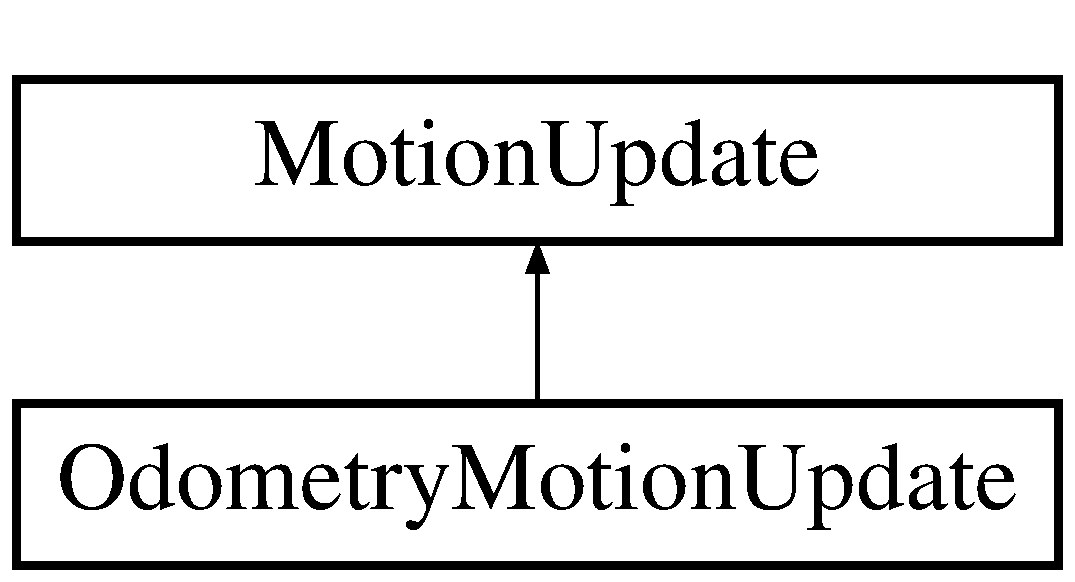
\includegraphics[height=2.000000cm]{classOdometryMotionUpdate}
\end{center}
\end{figure}
\subsection*{Public Member Functions}
\begin{DoxyCompactItemize}
\item 
\hypertarget{classOdometryMotionUpdate_aad5ced92f80ce30e6685837f8a593295}{\hyperlink{classOdometryMotionUpdate_aad5ced92f80ce30e6685837f8a593295}{Odometry\-Motion\-Update} ()}\label{classOdometryMotionUpdate_aad5ced92f80ce30e6685837f8a593295}

\begin{DoxyCompactList}\small\item\em Default Constructor. \end{DoxyCompactList}\item 
geometry\-\_\-msgs\-::\-Pose\-With\-Covariance\-Stamped \hyperlink{classOdometryMotionUpdate_aae9430006166324a62f4f7fbbd510841}{predict} (geometry\-\_\-msgs\-::\-Pose\-With\-Covariance\-Stamped pose, const nav\-\_\-msgs\-::\-Odometry\-::\-Const\-Ptr \&old\-\_\-msg, const nav\-\_\-msgs\-::\-Odometry\-::\-Const\-Ptr \&new\-\_\-msg)
\end{DoxyCompactItemize}
\subsection*{Additional Inherited Members}


\subsection{Detailed Description}
Odometry model implementation of motion update algorithm. 

\subsection{Member Function Documentation}
\hypertarget{classOdometryMotionUpdate_aae9430006166324a62f4f7fbbd510841}{\index{Odometry\-Motion\-Update@{Odometry\-Motion\-Update}!predict@{predict}}
\index{predict@{predict}!OdometryMotionUpdate@{Odometry\-Motion\-Update}}
\subsubsection[{predict}]{\setlength{\rightskip}{0pt plus 5cm}geometry\-\_\-msgs\-::\-Pose\-With\-Covariance\-Stamped Odometry\-Motion\-Update\-::predict (
\begin{DoxyParamCaption}
\item[{geometry\-\_\-msgs\-::\-Pose\-With\-Covariance\-Stamped}]{pose, }
\item[{const nav\-\_\-msgs\-::\-Odometry\-::\-Const\-Ptr \&}]{old\-\_\-msg, }
\item[{const nav\-\_\-msgs\-::\-Odometry\-::\-Const\-Ptr \&}]{new\-\_\-msg}
\end{DoxyParamCaption}
)\hspace{0.3cm}{\ttfamily [virtual]}}}\label{classOdometryMotionUpdate_aae9430006166324a62f4f7fbbd510841}
Predict the new pose. 
\begin{DoxyParams}{Parameters}
{\em pose} & current pose. \\
\hline
{\em old\-\_\-msg} & last odometry msg. \\
\hline
{\em new\-\_\-msg} & new odometry msg. \\
\hline
\end{DoxyParams}
\begin{DoxyReturn}{Returns}

\end{DoxyReturn}


Implements \hyperlink{classMotionUpdate_a86e028d43981218ddf6e354e8f201e75}{Motion\-Update}.



The documentation for this class was generated from the following file\-:\begin{DoxyCompactItemize}
\item 
include/localization/motion\-\_\-update\-\_\-strategies/\hyperlink{odometry__motion__update_8h}{odometry\-\_\-motion\-\_\-update.\-h}\end{DoxyCompactItemize}

\hypertarget{classParticle}{\section{Particle Class Reference}
\label{classParticle}\index{Particle@{Particle}}
}


Class that implements a particle for a S\-L\-A\-M algorithm.  




{\ttfamily \#include $<$particle.\-h$>$}

\subsection*{Public Member Functions}
\begin{DoxyCompactItemize}
\item 
\hypertarget{classParticle_a40f4c7e248029d72e7714b7802d5e5e1}{\hyperlink{classParticle_a40f4c7e248029d72e7714b7802d5e5e1}{Particle} ()}\label{classParticle_a40f4c7e248029d72e7714b7802d5e5e1}

\begin{DoxyCompactList}\small\item\em Default Constructor. \end{DoxyCompactList}\item 
\hyperlink{classParticle_ada5f546ca4314231550c84f4c80f58f1}{Particle} (double weight, geometry\-\_\-msgs\-::\-Pose\-With\-Covariance\-Stamped pose)
\item 
\hypertarget{classParticle_a2be6a5d2890263085642eff4b168fbbf}{double \hyperlink{classParticle_a2be6a5d2890263085642eff4b168fbbf}{get\-\_\-weight} ()}\label{classParticle_a2be6a5d2890263085642eff4b168fbbf}

\begin{DoxyCompactList}\small\item\em get particle belief \end{DoxyCompactList}\item 
\hypertarget{classParticle_ab6d40cebe007ecf4b4a979920e5b6812}{geometry\-\_\-msgs\-::\-Pose\-With\-Covariance\-Stamped \hyperlink{classParticle_ab6d40cebe007ecf4b4a979920e5b6812}{get\-\_\-pose} ()}\label{classParticle_ab6d40cebe007ecf4b4a979920e5b6812}

\begin{DoxyCompactList}\small\item\em get particle pose \end{DoxyCompactList}\item 
\hypertarget{classParticle_a59175592f7420c93a4d3e89da546473b}{\hyperlink{occupancy__map_8h_aea86d1b633e7d9b44b660a39fa9b50f7}{Occupancy\-Map\-Ptr} \hyperlink{classParticle_a59175592f7420c93a4d3e89da546473b}{get\-\_\-map} ()}\label{classParticle_a59175592f7420c93a4d3e89da546473b}

\begin{DoxyCompactList}\small\item\em get particle local map. \end{DoxyCompactList}\item 
void \hyperlink{classParticle_acd97e9df836f3f66f5a08a089a643c9a}{set\-\_\-weight} (double weight)
\item 
void \hyperlink{classParticle_a56f36d075622aa149afb833ded8dba51}{set\-\_\-pose} (geometry\-\_\-msgs\-::\-Pose\-With\-Covariance\-Stamped pose)
\item 
void \hyperlink{classParticle_a370b7228f1f7508cc1e768b1360c989e}{set\-\_\-map} (\hyperlink{occupancy__map_8h_aea86d1b633e7d9b44b660a39fa9b50f7}{Occupancy\-Map\-Ptr} map)
\end{DoxyCompactItemize}


\subsection{Detailed Description}
Class that implements a particle for a S\-L\-A\-M algorithm. 

\subsection{Constructor \& Destructor Documentation}
\hypertarget{classParticle_ada5f546ca4314231550c84f4c80f58f1}{\index{Particle@{Particle}!Particle@{Particle}}
\index{Particle@{Particle}!Particle@{Particle}}
\subsubsection[{Particle}]{\setlength{\rightskip}{0pt plus 5cm}Particle\-::\-Particle (
\begin{DoxyParamCaption}
\item[{double}]{weight, }
\item[{geometry\-\_\-msgs\-::\-Pose\-With\-Covariance\-Stamped}]{pose}
\end{DoxyParamCaption}
)}}\label{classParticle_ada5f546ca4314231550c84f4c80f58f1}
Class constructor. 
\begin{DoxyParams}{Parameters}
{\em weight} & particle belief. \\
\hline
{\em pose} & particle pose. \\
\hline
\end{DoxyParams}


\subsection{Member Function Documentation}
\hypertarget{classParticle_a370b7228f1f7508cc1e768b1360c989e}{\index{Particle@{Particle}!set\-\_\-map@{set\-\_\-map}}
\index{set\-\_\-map@{set\-\_\-map}!Particle@{Particle}}
\subsubsection[{set\-\_\-map}]{\setlength{\rightskip}{0pt plus 5cm}void Particle\-::set\-\_\-map (
\begin{DoxyParamCaption}
\item[{{\bf Occupancy\-Map\-Ptr}}]{map}
\end{DoxyParamCaption}
)}}\label{classParticle_a370b7228f1f7508cc1e768b1360c989e}
Set particle map 
\begin{DoxyParams}{Parameters}
{\em map} & \\
\hline
\end{DoxyParams}
\hypertarget{classParticle_a56f36d075622aa149afb833ded8dba51}{\index{Particle@{Particle}!set\-\_\-pose@{set\-\_\-pose}}
\index{set\-\_\-pose@{set\-\_\-pose}!Particle@{Particle}}
\subsubsection[{set\-\_\-pose}]{\setlength{\rightskip}{0pt plus 5cm}void Particle\-::set\-\_\-pose (
\begin{DoxyParamCaption}
\item[{geometry\-\_\-msgs\-::\-Pose\-With\-Covariance\-Stamped}]{pose}
\end{DoxyParamCaption}
)}}\label{classParticle_a56f36d075622aa149afb833ded8dba51}
Set particle pose 
\begin{DoxyParams}{Parameters}
{\em pose} & \\
\hline
\end{DoxyParams}
\hypertarget{classParticle_acd97e9df836f3f66f5a08a089a643c9a}{\index{Particle@{Particle}!set\-\_\-weight@{set\-\_\-weight}}
\index{set\-\_\-weight@{set\-\_\-weight}!Particle@{Particle}}
\subsubsection[{set\-\_\-weight}]{\setlength{\rightskip}{0pt plus 5cm}void Particle\-::set\-\_\-weight (
\begin{DoxyParamCaption}
\item[{double}]{weight}
\end{DoxyParamCaption}
)}}\label{classParticle_acd97e9df836f3f66f5a08a089a643c9a}
Set particle belief 
\begin{DoxyParams}{Parameters}
{\em weight} & \\
\hline
\end{DoxyParams}


The documentation for this class was generated from the following file\-:\begin{DoxyCompactItemize}
\item 
include/localization/util/\hyperlink{particle_8h}{particle.\-h}\end{DoxyCompactItemize}

\hypertarget{classParticleFilter}{\section{Particle\-Filter Class Reference}
\label{classParticleFilter}\index{Particle\-Filter@{Particle\-Filter}}
}


Implementation of the particle filter algorithm.  




{\ttfamily \#include $<$particle\-\_\-filter.\-h$>$}

Inheritance diagram for Particle\-Filter\-:\begin{figure}[H]
\begin{center}
\leavevmode
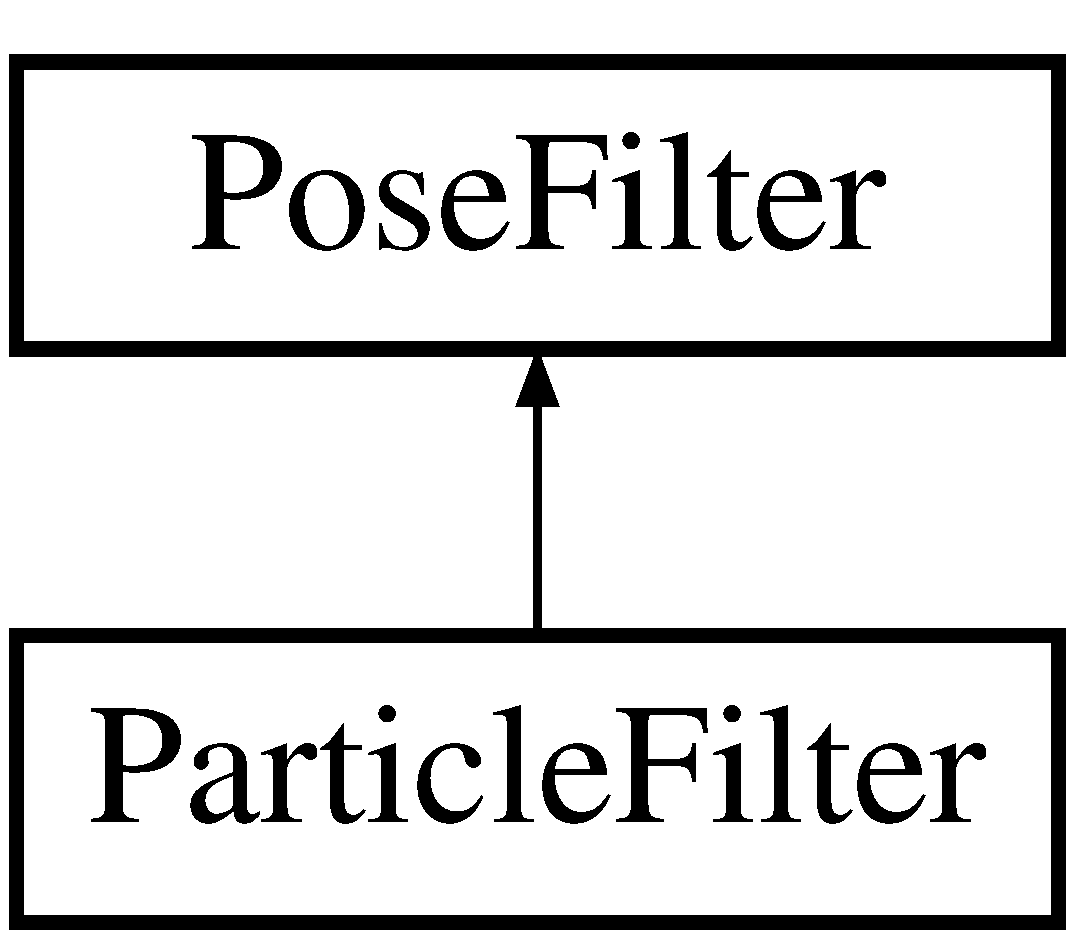
\includegraphics[height=2.000000cm]{classParticleFilter}
\end{center}
\end{figure}
\subsection*{Public Member Functions}
\begin{DoxyCompactItemize}
\item 
\hypertarget{classParticleFilter_ac5aeadcc4bf1f9f6a459562813e5b45f}{\hyperlink{classParticleFilter_ac5aeadcc4bf1f9f6a459562813e5b45f}{Particle\-Filter} ()}\label{classParticleFilter_ac5aeadcc4bf1f9f6a459562813e5b45f}

\begin{DoxyCompactList}\small\item\em Default Constructor. \end{DoxyCompactList}\item 
\hyperlink{classParticleFilter_aa1d16a1ae1d879c428e70e9c7ff62f00}{Particle\-Filter} (int number\-\_\-of\-\_\-particles, int random\-\_\-particles)
\item 
void \hyperlink{classParticleFilter_a111b1663c1865bd86e9f8666ebc88fb2}{motion\-\_\-update} (const nav\-\_\-msgs\-::\-Odometry\-::\-Const\-Ptr \&msg)
\item 
void \hyperlink{classParticleFilter_aa710931651bed02761e166cd77a49780}{sensor\-\_\-update} (const sensor\-\_\-msgs\-::\-Laser\-Scan\-::\-Const\-Ptr \&msg)
\item 
void \hyperlink{classParticleFilter_a84265f4c32f6d157da1d40677c6c47cf}{resample} ()
\item 
std\-::vector\\*
$<$ geometry\-\_\-msgs\-::\-Pose\-With\-Covariance\-Stamped $>$ \hyperlink{classParticleFilter_ac52e683f06369ef3e4741c5730db20d7}{get\-\_\-poses} ()
\item 
geometry\-\_\-msgs\-::\-Pose\-With\-Covariance\-Stamped \hyperlink{classParticleFilter_a7357ebc3eae177cead406c621940fe7c}{get\-\_\-best\-\_\-pose} ()
\item 
void \hyperlink{classParticleFilter_ab9a2cc375944db98ec7d6756660ae00e}{set\-\_\-map} (const nav\-\_\-msgs\-::\-Occupancy\-Grid\-::\-Const\-Ptr \&msg)
\item 
void \hyperlink{classParticleFilter_a789d8d5c9ccf81e10d5caa04fe11aa1a}{set\-\_\-number\-\_\-of\-\_\-particles} (int number\-\_\-of\-\_\-particles)
\item 
void \hyperlink{classParticleFilter_ac53de03b18934fa3cef2541497319bbe}{set\-\_\-random\-\_\-particles} (int random\-\_\-particles)
\item 
void \hyperlink{classParticleFilter_a6fa1de91f0c822573c6b9e0eac15050d}{reset\-\_\-particles} ()
\item 
std\-::vector$<$ \hyperlink{classParticle}{Particle} $>$ \hyperlink{classParticleFilter_a64c877049ce27490531fe0d437949929}{get\-\_\-particles} ()
\end{DoxyCompactItemize}
\subsection*{Additional Inherited Members}


\subsection{Detailed Description}
Implementation of the particle filter algorithm. 

\subsection{Constructor \& Destructor Documentation}
\hypertarget{classParticleFilter_aa1d16a1ae1d879c428e70e9c7ff62f00}{\index{Particle\-Filter@{Particle\-Filter}!Particle\-Filter@{Particle\-Filter}}
\index{Particle\-Filter@{Particle\-Filter}!ParticleFilter@{Particle\-Filter}}
\subsubsection[{Particle\-Filter}]{\setlength{\rightskip}{0pt plus 5cm}Particle\-Filter\-::\-Particle\-Filter (
\begin{DoxyParamCaption}
\item[{int}]{number\-\_\-of\-\_\-particles, }
\item[{int}]{random\-\_\-particles}
\end{DoxyParamCaption}
)}}\label{classParticleFilter_aa1d16a1ae1d879c428e70e9c7ff62f00}
Class constructor. 
\begin{DoxyParams}{Parameters}
{\em number\-\_\-of\-\_\-particles} & number of particles. \\
\hline
{\em random\-\_\-particles} & number of random particles to init in every iteration. \\
\hline
\end{DoxyParams}


\subsection{Member Function Documentation}
\hypertarget{classParticleFilter_a7357ebc3eae177cead406c621940fe7c}{\index{Particle\-Filter@{Particle\-Filter}!get\-\_\-best\-\_\-pose@{get\-\_\-best\-\_\-pose}}
\index{get\-\_\-best\-\_\-pose@{get\-\_\-best\-\_\-pose}!ParticleFilter@{Particle\-Filter}}
\subsubsection[{get\-\_\-best\-\_\-pose}]{\setlength{\rightskip}{0pt plus 5cm}geometry\-\_\-msgs\-::\-Pose\-With\-Covariance\-Stamped Particle\-Filter\-::get\-\_\-best\-\_\-pose (
\begin{DoxyParamCaption}
{}
\end{DoxyParamCaption}
)\hspace{0.3cm}{\ttfamily [virtual]}}}\label{classParticleFilter_a7357ebc3eae177cead406c621940fe7c}
Get the best pose \begin{DoxyReturn}{Returns}
pose with covariance 
\end{DoxyReturn}


Implements \hyperlink{classPoseFilter_a64686b9d07bd339cdd7c269b4c173404}{Pose\-Filter}.

\hypertarget{classParticleFilter_a64c877049ce27490531fe0d437949929}{\index{Particle\-Filter@{Particle\-Filter}!get\-\_\-particles@{get\-\_\-particles}}
\index{get\-\_\-particles@{get\-\_\-particles}!ParticleFilter@{Particle\-Filter}}
\subsubsection[{get\-\_\-particles}]{\setlength{\rightskip}{0pt plus 5cm}std\-::vector$<${\bf Particle}$>$ Particle\-Filter\-::get\-\_\-particles (
\begin{DoxyParamCaption}
{}
\end{DoxyParamCaption}
)}}\label{classParticleFilter_a64c877049ce27490531fe0d437949929}
Get the particles. \begin{DoxyReturn}{Returns}
vector of particles. 
\end{DoxyReturn}
\hypertarget{classParticleFilter_ac52e683f06369ef3e4741c5730db20d7}{\index{Particle\-Filter@{Particle\-Filter}!get\-\_\-poses@{get\-\_\-poses}}
\index{get\-\_\-poses@{get\-\_\-poses}!ParticleFilter@{Particle\-Filter}}
\subsubsection[{get\-\_\-poses}]{\setlength{\rightskip}{0pt plus 5cm}std\-::vector$<$geometry\-\_\-msgs\-::\-Pose\-With\-Covariance\-Stamped$>$ Particle\-Filter\-::get\-\_\-poses (
\begin{DoxyParamCaption}
{}
\end{DoxyParamCaption}
)\hspace{0.3cm}{\ttfamily [virtual]}}}\label{classParticleFilter_ac52e683f06369ef3e4741c5730db20d7}
Retrieve the estimated poses \begin{DoxyReturn}{Returns}
vector of poses with covariances. 
\end{DoxyReturn}


Implements \hyperlink{classPoseFilter_af84e0ef9dbca4892408930383acbe810}{Pose\-Filter}.

\hypertarget{classParticleFilter_a111b1663c1865bd86e9f8666ebc88fb2}{\index{Particle\-Filter@{Particle\-Filter}!motion\-\_\-update@{motion\-\_\-update}}
\index{motion\-\_\-update@{motion\-\_\-update}!ParticleFilter@{Particle\-Filter}}
\subsubsection[{motion\-\_\-update}]{\setlength{\rightskip}{0pt plus 5cm}void Particle\-Filter\-::motion\-\_\-update (
\begin{DoxyParamCaption}
\item[{const nav\-\_\-msgs\-::\-Odometry\-::\-Const\-Ptr \&}]{msg}
\end{DoxyParamCaption}
)\hspace{0.3cm}{\ttfamily [virtual]}}}\label{classParticleFilter_a111b1663c1865bd86e9f8666ebc88fb2}
Execute motion update step. 
\begin{DoxyParams}{Parameters}
{\em msg} & odometry msg pointer. \\
\hline
\end{DoxyParams}


Implements \hyperlink{classPoseFilter_ad40e8f2ae14a14211f3729a4869e312d}{Pose\-Filter}.

\hypertarget{classParticleFilter_a84265f4c32f6d157da1d40677c6c47cf}{\index{Particle\-Filter@{Particle\-Filter}!resample@{resample}}
\index{resample@{resample}!ParticleFilter@{Particle\-Filter}}
\subsubsection[{resample}]{\setlength{\rightskip}{0pt plus 5cm}void Particle\-Filter\-::resample (
\begin{DoxyParamCaption}
{}
\end{DoxyParamCaption}
)}}\label{classParticleFilter_a84265f4c32f6d157da1d40677c6c47cf}
Execute resampling algorithm \hypertarget{classParticleFilter_a6fa1de91f0c822573c6b9e0eac15050d}{\index{Particle\-Filter@{Particle\-Filter}!reset\-\_\-particles@{reset\-\_\-particles}}
\index{reset\-\_\-particles@{reset\-\_\-particles}!ParticleFilter@{Particle\-Filter}}
\subsubsection[{reset\-\_\-particles}]{\setlength{\rightskip}{0pt plus 5cm}void Particle\-Filter\-::reset\-\_\-particles (
\begin{DoxyParamCaption}
{}
\end{DoxyParamCaption}
)}}\label{classParticleFilter_a6fa1de91f0c822573c6b9e0eac15050d}
Reset the particles. \hypertarget{classParticleFilter_aa710931651bed02761e166cd77a49780}{\index{Particle\-Filter@{Particle\-Filter}!sensor\-\_\-update@{sensor\-\_\-update}}
\index{sensor\-\_\-update@{sensor\-\_\-update}!ParticleFilter@{Particle\-Filter}}
\subsubsection[{sensor\-\_\-update}]{\setlength{\rightskip}{0pt plus 5cm}void Particle\-Filter\-::sensor\-\_\-update (
\begin{DoxyParamCaption}
\item[{const sensor\-\_\-msgs\-::\-Laser\-Scan\-::\-Const\-Ptr \&}]{msg}
\end{DoxyParamCaption}
)\hspace{0.3cm}{\ttfamily [virtual]}}}\label{classParticleFilter_aa710931651bed02761e166cd77a49780}
Execute sensor correcting step. 
\begin{DoxyParams}{Parameters}
{\em msg} & laser msg pointer. \\
\hline
\end{DoxyParams}


Implements \hyperlink{classPoseFilter_a42d8e867c65b45894f934d7b2c60b684}{Pose\-Filter}.

\hypertarget{classParticleFilter_ab9a2cc375944db98ec7d6756660ae00e}{\index{Particle\-Filter@{Particle\-Filter}!set\-\_\-map@{set\-\_\-map}}
\index{set\-\_\-map@{set\-\_\-map}!ParticleFilter@{Particle\-Filter}}
\subsubsection[{set\-\_\-map}]{\setlength{\rightskip}{0pt plus 5cm}void Particle\-Filter\-::set\-\_\-map (
\begin{DoxyParamCaption}
\item[{const nav\-\_\-msgs\-::\-Occupancy\-Grid\-::\-Const\-Ptr \&}]{msg}
\end{DoxyParamCaption}
)\hspace{0.3cm}{\ttfamily [virtual]}}}\label{classParticleFilter_ab9a2cc375944db98ec7d6756660ae00e}
Set map to the algorithm 
\begin{DoxyParams}{Parameters}
{\em msg} & occupancy grid msg pointer. \\
\hline
\end{DoxyParams}


Reimplemented from \hyperlink{classPoseFilter_ab5a6b461992f3ce218b308a59f50a83f}{Pose\-Filter}.

\hypertarget{classParticleFilter_a789d8d5c9ccf81e10d5caa04fe11aa1a}{\index{Particle\-Filter@{Particle\-Filter}!set\-\_\-number\-\_\-of\-\_\-particles@{set\-\_\-number\-\_\-of\-\_\-particles}}
\index{set\-\_\-number\-\_\-of\-\_\-particles@{set\-\_\-number\-\_\-of\-\_\-particles}!ParticleFilter@{Particle\-Filter}}
\subsubsection[{set\-\_\-number\-\_\-of\-\_\-particles}]{\setlength{\rightskip}{0pt plus 5cm}void Particle\-Filter\-::set\-\_\-number\-\_\-of\-\_\-particles (
\begin{DoxyParamCaption}
\item[{int}]{number\-\_\-of\-\_\-particles}
\end{DoxyParamCaption}
)}}\label{classParticleFilter_a789d8d5c9ccf81e10d5caa04fe11aa1a}
Set the number of particles to the algorithm. 
\begin{DoxyParams}{Parameters}
{\em number\-\_\-of\-\_\-particles} & \\
\hline
\end{DoxyParams}
\hypertarget{classParticleFilter_ac53de03b18934fa3cef2541497319bbe}{\index{Particle\-Filter@{Particle\-Filter}!set\-\_\-random\-\_\-particles@{set\-\_\-random\-\_\-particles}}
\index{set\-\_\-random\-\_\-particles@{set\-\_\-random\-\_\-particles}!ParticleFilter@{Particle\-Filter}}
\subsubsection[{set\-\_\-random\-\_\-particles}]{\setlength{\rightskip}{0pt plus 5cm}void Particle\-Filter\-::set\-\_\-random\-\_\-particles (
\begin{DoxyParamCaption}
\item[{int}]{random\-\_\-particles}
\end{DoxyParamCaption}
)}}\label{classParticleFilter_ac53de03b18934fa3cef2541497319bbe}
Set the number of random particles to be reset in each iteration. 
\begin{DoxyParams}{Parameters}
{\em random\-\_\-particles} & \\
\hline
\end{DoxyParams}


The documentation for this class was generated from the following file\-:\begin{DoxyCompactItemize}
\item 
include/localization/filtering\-\_\-strategies/\hyperlink{particle__filter_8h}{particle\-\_\-filter.\-h}\end{DoxyCompactItemize}

\hypertarget{classPoseFilter}{\section{Pose\-Filter Class Reference}
\label{classPoseFilter}\index{Pose\-Filter@{Pose\-Filter}}
}


Abstract class for implementing the pose filter strategy pattern.  




{\ttfamily \#include $<$pose\-\_\-filter.\-h$>$}

Inheritance diagram for Pose\-Filter\-:\begin{figure}[H]
\begin{center}
\leavevmode
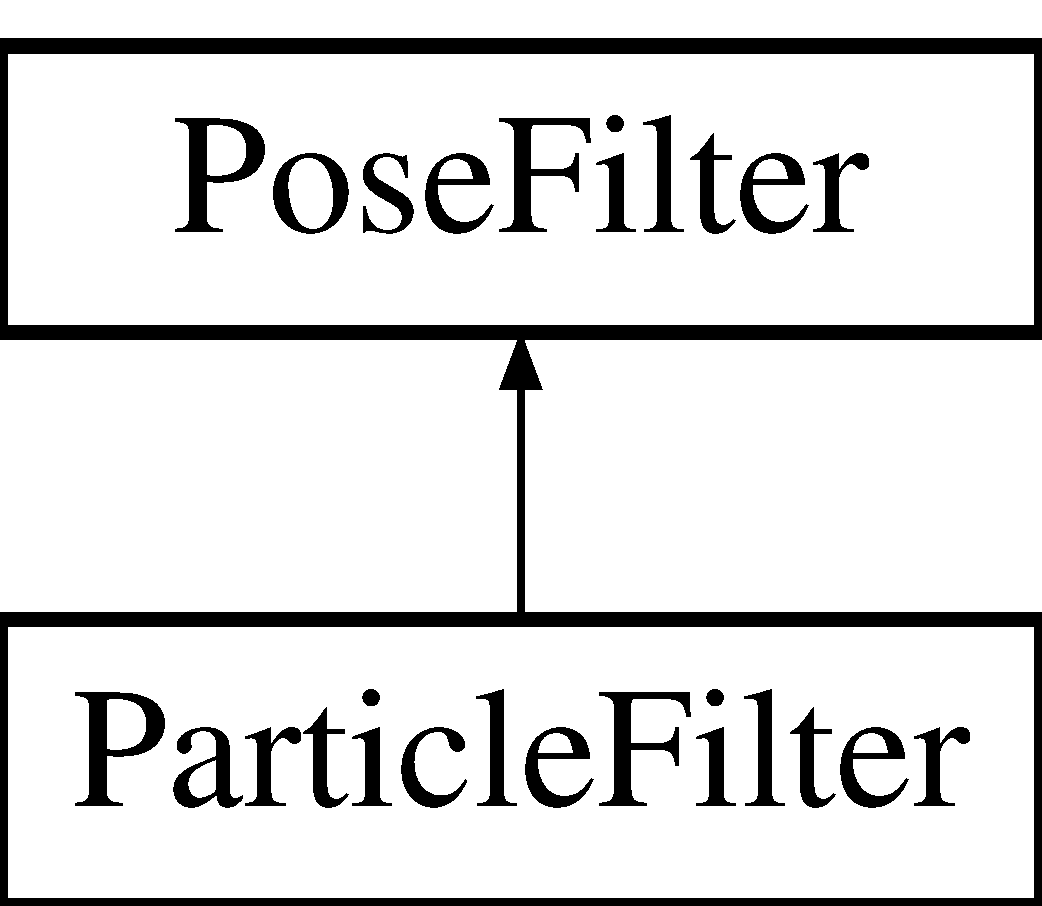
\includegraphics[height=2.000000cm]{classPoseFilter}
\end{center}
\end{figure}
\subsection*{Public Member Functions}
\begin{DoxyCompactItemize}
\item 
virtual void \hyperlink{classPoseFilter_ad40e8f2ae14a14211f3729a4869e312d}{motion\-\_\-update} (const nav\-\_\-msgs\-::\-Odometry\-::\-Const\-Ptr \&msg)=0
\begin{DoxyCompactList}\small\item\em Virtual Destructor. \end{DoxyCompactList}\item 
virtual void \hyperlink{classPoseFilter_a42d8e867c65b45894f934d7b2c60b684}{sensor\-\_\-update} (const sensor\-\_\-msgs\-::\-Laser\-Scan\-::\-Const\-Ptr \&msg)=0
\item 
virtual std\-::vector\\*
$<$ geometry\-\_\-msgs\-::\-Pose\-With\-Covariance\-Stamped $>$ \hyperlink{classPoseFilter_af84e0ef9dbca4892408930383acbe810}{get\-\_\-poses} ()=0
\item 
virtual \\*
geometry\-\_\-msgs\-::\-Pose\-With\-Covariance\-Stamped \hyperlink{classPoseFilter_a64686b9d07bd339cdd7c269b4c173404}{get\-\_\-best\-\_\-pose} ()=0
\item 
void \hyperlink{classPoseFilter_aef63acc2ba1bf411909cae2992a90c7d}{set\-\_\-motion\-\_\-update\-\_\-strategy} (\hyperlink{motion__update_8h_aec1cf0d54c70c4dacac639ab488bf948}{Motion\-Update\-Ptr} ptr)
\item 
void \hyperlink{classPoseFilter_a771670fb9bcbbab0964a7310343b2201}{set\-\_\-sensor\-\_\-update\-\_\-strategy} (\hyperlink{sensor__update_8h_a7bfe6ec1a05f2f99b0974d5cbd8b8b7b}{Sensor\-Update\-Ptr} ptr)
\item 
void \hyperlink{classPoseFilter_af9c8fa9dcbe05ae4be64823d894e6514}{set\-\_\-sampling\-\_\-strategy} (\hyperlink{sampling_8h_adf4afed667a21b30f8ff816aae609bf7}{Sampling\-Ptr} ptr)
\item 
virtual void \hyperlink{classPoseFilter_ab5a6b461992f3ce218b308a59f50a83f}{set\-\_\-map} (const nav\-\_\-msgs\-::\-Occupancy\-Grid\-::\-Const\-Ptr \&msg)
\item 
std\-::string \hyperlink{classPoseFilter_a7536e09a70e3683a8de5c94b9a1b5a53}{get\-\_\-name} ()
\item 
std\-::string \hyperlink{classPoseFilter_a566fe40b9b00a6ebedfb615acaf80142}{get\-\_\-frame} ()
\end{DoxyCompactItemize}
\subsection*{Protected Attributes}
\begin{DoxyCompactItemize}
\item 
\hypertarget{classPoseFilter_a4cfce1dfd10de209e15ba5788a96ba73}{std\-::string \hyperlink{classPoseFilter_a4cfce1dfd10de209e15ba5788a96ba73}{\-\_\-name}}\label{classPoseFilter_a4cfce1dfd10de209e15ba5788a96ba73}

\begin{DoxyCompactList}\small\item\em algorithm name. \end{DoxyCompactList}\item 
\hypertarget{classPoseFilter_a67e475eebbfbde4da3e357c698b29ebb}{\hyperlink{motion__update_8h_aec1cf0d54c70c4dacac639ab488bf948}{Motion\-Update\-Ptr} \hyperlink{classPoseFilter_a67e475eebbfbde4da3e357c698b29ebb}{\-\_\-motion\-\_\-update\-\_\-strategy}}\label{classPoseFilter_a67e475eebbfbde4da3e357c698b29ebb}

\begin{DoxyCompactList}\small\item\em motion update model. \end{DoxyCompactList}\item 
\hypertarget{classPoseFilter_aa2a032edfb970eb65323febc69f1d722}{\hyperlink{sensor__update_8h_a7bfe6ec1a05f2f99b0974d5cbd8b8b7b}{Sensor\-Update\-Ptr} \hyperlink{classPoseFilter_aa2a032edfb970eb65323febc69f1d722}{\-\_\-sensor\-\_\-update\-\_\-strategy}}\label{classPoseFilter_aa2a032edfb970eb65323febc69f1d722}

\begin{DoxyCompactList}\small\item\em sensor update model. \end{DoxyCompactList}\item 
\hypertarget{classPoseFilter_a7abb5e0250adde708d72937b982d87db}{\hyperlink{sampling_8h_adf4afed667a21b30f8ff816aae609bf7}{Sampling\-Ptr} \hyperlink{classPoseFilter_a7abb5e0250adde708d72937b982d87db}{\-\_\-sampling\-\_\-strategy}}\label{classPoseFilter_a7abb5e0250adde708d72937b982d87db}

\begin{DoxyCompactList}\small\item\em sampling strategy model. \end{DoxyCompactList}\item 
\hypertarget{classPoseFilter_a3412c99421ee59cf13fe0d627b31a400}{nav\-\_\-msgs\-::\-Occupancy\-Grid \hyperlink{classPoseFilter_a3412c99421ee59cf13fe0d627b31a400}{\-\_\-map}}\label{classPoseFilter_a3412c99421ee59cf13fe0d627b31a400}

\begin{DoxyCompactList}\small\item\em global map model. \end{DoxyCompactList}\item 
\hypertarget{classPoseFilter_a1399dd6813d7c853181bd98024a2cfe0}{bool \hyperlink{classPoseFilter_a1399dd6813d7c853181bd98024a2cfe0}{\-\_\-is\-\_\-map\-\_\-set}}\label{classPoseFilter_a1399dd6813d7c853181bd98024a2cfe0}

\begin{DoxyCompactList}\small\item\em boolean to check if map is set. \end{DoxyCompactList}\end{DoxyCompactItemize}


\subsection{Detailed Description}
Abstract class for implementing the pose filter strategy pattern. 

\subsection{Member Function Documentation}
\hypertarget{classPoseFilter_a64686b9d07bd339cdd7c269b4c173404}{\index{Pose\-Filter@{Pose\-Filter}!get\-\_\-best\-\_\-pose@{get\-\_\-best\-\_\-pose}}
\index{get\-\_\-best\-\_\-pose@{get\-\_\-best\-\_\-pose}!PoseFilter@{Pose\-Filter}}
\subsubsection[{get\-\_\-best\-\_\-pose}]{\setlength{\rightskip}{0pt plus 5cm}virtual geometry\-\_\-msgs\-::\-Pose\-With\-Covariance\-Stamped Pose\-Filter\-::get\-\_\-best\-\_\-pose (
\begin{DoxyParamCaption}
{}
\end{DoxyParamCaption}
)\hspace{0.3cm}{\ttfamily [pure virtual]}}}\label{classPoseFilter_a64686b9d07bd339cdd7c269b4c173404}
Get the best estimation of the pose. \begin{DoxyReturn}{Returns}

\end{DoxyReturn}


Implemented in \hyperlink{classParticleFilter_a7357ebc3eae177cead406c621940fe7c}{Particle\-Filter}.

\hypertarget{classPoseFilter_a566fe40b9b00a6ebedfb615acaf80142}{\index{Pose\-Filter@{Pose\-Filter}!get\-\_\-frame@{get\-\_\-frame}}
\index{get\-\_\-frame@{get\-\_\-frame}!PoseFilter@{Pose\-Filter}}
\subsubsection[{get\-\_\-frame}]{\setlength{\rightskip}{0pt plus 5cm}std\-::string Pose\-Filter\-::get\-\_\-frame (
\begin{DoxyParamCaption}
{}
\end{DoxyParamCaption}
)}}\label{classPoseFilter_a566fe40b9b00a6ebedfb615acaf80142}
Return algorithm reference frame. \begin{DoxyReturn}{Returns}

\end{DoxyReturn}
\hypertarget{classPoseFilter_a7536e09a70e3683a8de5c94b9a1b5a53}{\index{Pose\-Filter@{Pose\-Filter}!get\-\_\-name@{get\-\_\-name}}
\index{get\-\_\-name@{get\-\_\-name}!PoseFilter@{Pose\-Filter}}
\subsubsection[{get\-\_\-name}]{\setlength{\rightskip}{0pt plus 5cm}std\-::string Pose\-Filter\-::get\-\_\-name (
\begin{DoxyParamCaption}
{}
\end{DoxyParamCaption}
)}}\label{classPoseFilter_a7536e09a70e3683a8de5c94b9a1b5a53}
Return algorithm name. \begin{DoxyReturn}{Returns}

\end{DoxyReturn}
\hypertarget{classPoseFilter_af84e0ef9dbca4892408930383acbe810}{\index{Pose\-Filter@{Pose\-Filter}!get\-\_\-poses@{get\-\_\-poses}}
\index{get\-\_\-poses@{get\-\_\-poses}!PoseFilter@{Pose\-Filter}}
\subsubsection[{get\-\_\-poses}]{\setlength{\rightskip}{0pt plus 5cm}virtual std\-::vector$<$geometry\-\_\-msgs\-::\-Pose\-With\-Covariance\-Stamped$>$ Pose\-Filter\-::get\-\_\-poses (
\begin{DoxyParamCaption}
{}
\end{DoxyParamCaption}
)\hspace{0.3cm}{\ttfamily [pure virtual]}}}\label{classPoseFilter_af84e0ef9dbca4892408930383acbe810}
Get all the estimated poses. \begin{DoxyReturn}{Returns}

\end{DoxyReturn}


Implemented in \hyperlink{classParticleFilter_ac52e683f06369ef3e4741c5730db20d7}{Particle\-Filter}.

\hypertarget{classPoseFilter_ad40e8f2ae14a14211f3729a4869e312d}{\index{Pose\-Filter@{Pose\-Filter}!motion\-\_\-update@{motion\-\_\-update}}
\index{motion\-\_\-update@{motion\-\_\-update}!PoseFilter@{Pose\-Filter}}
\subsubsection[{motion\-\_\-update}]{\setlength{\rightskip}{0pt plus 5cm}virtual void Pose\-Filter\-::motion\-\_\-update (
\begin{DoxyParamCaption}
\item[{const nav\-\_\-msgs\-::\-Odometry\-::\-Const\-Ptr \&}]{msg}
\end{DoxyParamCaption}
)\hspace{0.3cm}{\ttfamily [pure virtual]}}}\label{classPoseFilter_ad40e8f2ae14a14211f3729a4869e312d}


Virtual Destructor. 

Execute motion update step. 
\begin{DoxyParams}{Parameters}
{\em msg} & odometry msg pointer. \\
\hline
\end{DoxyParams}


Implemented in \hyperlink{classParticleFilter_a111b1663c1865bd86e9f8666ebc88fb2}{Particle\-Filter}.

\hypertarget{classPoseFilter_a42d8e867c65b45894f934d7b2c60b684}{\index{Pose\-Filter@{Pose\-Filter}!sensor\-\_\-update@{sensor\-\_\-update}}
\index{sensor\-\_\-update@{sensor\-\_\-update}!PoseFilter@{Pose\-Filter}}
\subsubsection[{sensor\-\_\-update}]{\setlength{\rightskip}{0pt plus 5cm}virtual void Pose\-Filter\-::sensor\-\_\-update (
\begin{DoxyParamCaption}
\item[{const sensor\-\_\-msgs\-::\-Laser\-Scan\-::\-Const\-Ptr \&}]{msg}
\end{DoxyParamCaption}
)\hspace{0.3cm}{\ttfamily [pure virtual]}}}\label{classPoseFilter_a42d8e867c65b45894f934d7b2c60b684}
Execute sensor correcting step. 
\begin{DoxyParams}{Parameters}
{\em msg} & laser msg pointer. \\
\hline
\end{DoxyParams}


Implemented in \hyperlink{classParticleFilter_aa710931651bed02761e166cd77a49780}{Particle\-Filter}.

\hypertarget{classPoseFilter_ab5a6b461992f3ce218b308a59f50a83f}{\index{Pose\-Filter@{Pose\-Filter}!set\-\_\-map@{set\-\_\-map}}
\index{set\-\_\-map@{set\-\_\-map}!PoseFilter@{Pose\-Filter}}
\subsubsection[{set\-\_\-map}]{\setlength{\rightskip}{0pt plus 5cm}void Pose\-Filter\-::set\-\_\-map (
\begin{DoxyParamCaption}
\item[{const nav\-\_\-msgs\-::\-Occupancy\-Grid\-::\-Const\-Ptr \&}]{msg}
\end{DoxyParamCaption}
)\hspace{0.3cm}{\ttfamily [virtual]}}}\label{classPoseFilter_ab5a6b461992f3ce218b308a59f50a83f}
Set map to the algorithm 
\begin{DoxyParams}{Parameters}
{\em msg} & occupancy grid msg pointer. \\
\hline
\end{DoxyParams}


Reimplemented in \hyperlink{classParticleFilter_ab9a2cc375944db98ec7d6756660ae00e}{Particle\-Filter}.

\hypertarget{classPoseFilter_aef63acc2ba1bf411909cae2992a90c7d}{\index{Pose\-Filter@{Pose\-Filter}!set\-\_\-motion\-\_\-update\-\_\-strategy@{set\-\_\-motion\-\_\-update\-\_\-strategy}}
\index{set\-\_\-motion\-\_\-update\-\_\-strategy@{set\-\_\-motion\-\_\-update\-\_\-strategy}!PoseFilter@{Pose\-Filter}}
\subsubsection[{set\-\_\-motion\-\_\-update\-\_\-strategy}]{\setlength{\rightskip}{0pt plus 5cm}void Pose\-Filter\-::set\-\_\-motion\-\_\-update\-\_\-strategy (
\begin{DoxyParamCaption}
\item[{{\bf Motion\-Update\-Ptr}}]{ptr}
\end{DoxyParamCaption}
)}}\label{classPoseFilter_aef63acc2ba1bf411909cae2992a90c7d}
Set the motion model implementation. 
\begin{DoxyParams}{Parameters}
{\em ptr} & motion update pointer. \\
\hline
\end{DoxyParams}
\hypertarget{classPoseFilter_af9c8fa9dcbe05ae4be64823d894e6514}{\index{Pose\-Filter@{Pose\-Filter}!set\-\_\-sampling\-\_\-strategy@{set\-\_\-sampling\-\_\-strategy}}
\index{set\-\_\-sampling\-\_\-strategy@{set\-\_\-sampling\-\_\-strategy}!PoseFilter@{Pose\-Filter}}
\subsubsection[{set\-\_\-sampling\-\_\-strategy}]{\setlength{\rightskip}{0pt plus 5cm}void Pose\-Filter\-::set\-\_\-sampling\-\_\-strategy (
\begin{DoxyParamCaption}
\item[{{\bf Sampling\-Ptr}}]{ptr}
\end{DoxyParamCaption}
)}}\label{classPoseFilter_af9c8fa9dcbe05ae4be64823d894e6514}
Set the sampling strategy implementation. 
\begin{DoxyParams}{Parameters}
{\em ptr} & sampling strategy pointer. \\
\hline
\end{DoxyParams}
\hypertarget{classPoseFilter_a771670fb9bcbbab0964a7310343b2201}{\index{Pose\-Filter@{Pose\-Filter}!set\-\_\-sensor\-\_\-update\-\_\-strategy@{set\-\_\-sensor\-\_\-update\-\_\-strategy}}
\index{set\-\_\-sensor\-\_\-update\-\_\-strategy@{set\-\_\-sensor\-\_\-update\-\_\-strategy}!PoseFilter@{Pose\-Filter}}
\subsubsection[{set\-\_\-sensor\-\_\-update\-\_\-strategy}]{\setlength{\rightskip}{0pt plus 5cm}void Pose\-Filter\-::set\-\_\-sensor\-\_\-update\-\_\-strategy (
\begin{DoxyParamCaption}
\item[{{\bf Sensor\-Update\-Ptr}}]{ptr}
\end{DoxyParamCaption}
)}}\label{classPoseFilter_a771670fb9bcbbab0964a7310343b2201}
Set the sensor model implementation. 
\begin{DoxyParams}{Parameters}
{\em ptr} & sensor update pointer. \\
\hline
\end{DoxyParams}


The documentation for this class was generated from the following files\-:\begin{DoxyCompactItemize}
\item 
include/localization/filtering\-\_\-strategies/\hyperlink{pose__filter_8h}{pose\-\_\-filter.\-h}\item 
include/localization/filtering\-\_\-strategies/\hyperlink{pose__filter_8hpp}{pose\-\_\-filter.\-hpp}\end{DoxyCompactItemize}

\hypertarget{classRosParameterParser}{\section{Ros\-Parameter\-Parser Class Reference}
\label{classRosParameterParser}\index{Ros\-Parameter\-Parser@{Ros\-Parameter\-Parser}}
}


Class that parses all parameters from R\-O\-S parameter server.  




{\ttfamily \#include $<$ros\-\_\-parameter\-\_\-parser.\-h$>$}

\subsection*{Public Member Functions}
\begin{DoxyCompactItemize}
\item 
\hypertarget{classRosParameterParser_aa1eaced586a61c482cc60e48d3da031a}{\hyperlink{classRosParameterParser_aa1eaced586a61c482cc60e48d3da031a}{Ros\-Parameter\-Parser} (ros\-::\-Node\-Handle nh)}\label{classRosParameterParser_aa1eaced586a61c482cc60e48d3da031a}

\begin{DoxyCompactList}\small\item\em Default Constructor. \end{DoxyCompactList}\item 
\hypertarget{classRosParameterParser_a06db85a3ac12b1fa6c2efd22a884d529}{\hyperlink{pose__filter_8h_a9df59d7c2f322f00bdd8eccab6d3fd73}{Pose\-Filter\-Ptr} \hyperlink{classRosParameterParser_a06db85a3ac12b1fa6c2efd22a884d529}{get\-\_\-filter} ()}\label{classRosParameterParser_a06db85a3ac12b1fa6c2efd22a884d529}

\begin{DoxyCompactList}\small\item\em Get parsed filter strategy implementation. \end{DoxyCompactList}\item 
\hypertarget{classRosParameterParser_a30f4b5a22749c66c26eb2b7854112d0d}{\hyperlink{motion__update_8h_aec1cf0d54c70c4dacac639ab488bf948}{Motion\-Update\-Ptr} \hyperlink{classRosParameterParser_a30f4b5a22749c66c26eb2b7854112d0d}{get\-\_\-motion\-\_\-update} ()}\label{classRosParameterParser_a30f4b5a22749c66c26eb2b7854112d0d}

\begin{DoxyCompactList}\small\item\em Get parsed motion update strategy implementation. \end{DoxyCompactList}\item 
\hypertarget{classRosParameterParser_aaf3ecb33630fecb04fc0088abb60e4c1}{\hyperlink{sensor__update_8h_a7bfe6ec1a05f2f99b0974d5cbd8b8b7b}{Sensor\-Update\-Ptr} \hyperlink{classRosParameterParser_aaf3ecb33630fecb04fc0088abb60e4c1}{get\-\_\-sensor\-\_\-update} ()}\label{classRosParameterParser_aaf3ecb33630fecb04fc0088abb60e4c1}

\begin{DoxyCompactList}\small\item\em Get parsed sensor update strategy implementation. \end{DoxyCompactList}\item 
\hypertarget{classRosParameterParser_ab29100583b22886d2c4158820253a515}{\hyperlink{sampling_8h_adf4afed667a21b30f8ff816aae609bf7}{Sampling\-Ptr} \hyperlink{classRosParameterParser_ab29100583b22886d2c4158820253a515}{get\-\_\-sampling\-\_\-strategy} ()}\label{classRosParameterParser_ab29100583b22886d2c4158820253a515}

\begin{DoxyCompactList}\small\item\em Get parsed sampling strategy implementation. \end{DoxyCompactList}\end{DoxyCompactItemize}


\subsection{Detailed Description}
Class that parses all parameters from R\-O\-S parameter server. 

The documentation for this class was generated from the following file\-:\begin{DoxyCompactItemize}
\item 
include/localization/parsers/\hyperlink{ros__parameter__parser_8h}{ros\-\_\-parameter\-\_\-parser.\-h}\end{DoxyCompactItemize}

\hypertarget{classRosTopicParser}{\section{Ros\-Topic\-Parser Class Reference}
\label{classRosTopicParser}\index{Ros\-Topic\-Parser@{Ros\-Topic\-Parser}}
}


Class that parses all topics from R\-O\-S parameter server.  




{\ttfamily \#include $<$ros\-\_\-topic\-\_\-parser.\-h$>$}

\subsection*{Public Member Functions}
\begin{DoxyCompactItemize}
\item 
\hyperlink{classRosTopicParser_a99ed0a18a0184c77830a5039892d4722}{Ros\-Topic\-Parser} (ros\-::\-Node\-Handle nh, std\-::string topic)
\item 
\hypertarget{classRosTopicParser_aea4a849f4cbb7825aa72aad390ac261c}{std\-::string \hyperlink{classRosTopicParser_aea4a849f4cbb7825aa72aad390ac261c}{get\-\_\-topic\-\_\-name} ()}\label{classRosTopicParser_aea4a849f4cbb7825aa72aad390ac261c}

\begin{DoxyCompactList}\small\item\em Get parsed topic name. \end{DoxyCompactList}\item 
\hypertarget{classRosTopicParser_a807bc6a064e91c0731b946ce6d10ccf2}{int \hyperlink{classRosTopicParser_a807bc6a064e91c0731b946ce6d10ccf2}{get\-\_\-queue\-\_\-size} ()}\label{classRosTopicParser_a807bc6a064e91c0731b946ce6d10ccf2}

\begin{DoxyCompactList}\small\item\em Get parsed topic queue size. \end{DoxyCompactList}\end{DoxyCompactItemize}


\subsection{Detailed Description}
Class that parses all topics from R\-O\-S parameter server. 

\subsection{Constructor \& Destructor Documentation}
\hypertarget{classRosTopicParser_a99ed0a18a0184c77830a5039892d4722}{\index{Ros\-Topic\-Parser@{Ros\-Topic\-Parser}!Ros\-Topic\-Parser@{Ros\-Topic\-Parser}}
\index{Ros\-Topic\-Parser@{Ros\-Topic\-Parser}!RosTopicParser@{Ros\-Topic\-Parser}}
\subsubsection[{Ros\-Topic\-Parser}]{\setlength{\rightskip}{0pt plus 5cm}Ros\-Topic\-Parser\-::\-Ros\-Topic\-Parser (
\begin{DoxyParamCaption}
\item[{ros\-::\-Node\-Handle}]{nh, }
\item[{std\-::string}]{topic}
\end{DoxyParamCaption}
)}}\label{classRosTopicParser_a99ed0a18a0184c77830a5039892d4722}
Parser constructor 
\begin{DoxyParams}{Parameters}
{\em nh} & ros node handler \\
\hline
{\em topic} & topic to be parsed \\
\hline
\end{DoxyParams}


The documentation for this class was generated from the following file\-:\begin{DoxyCompactItemize}
\item 
include/localization/parsers/\hyperlink{ros__topic__parser_8h}{ros\-\_\-topic\-\_\-parser.\-h}\end{DoxyCompactItemize}

\hypertarget{classRouletteWheelSampling}{\section{Roulette\-Wheel\-Sampling Class Reference}
\label{classRouletteWheelSampling}\index{Roulette\-Wheel\-Sampling@{Roulette\-Wheel\-Sampling}}
}


Roulette wheel implementation of sampling strategy pattern for particles.  




{\ttfamily \#include $<$roulette\-\_\-wheel\-\_\-sampling.\-h$>$}

Inheritance diagram for Roulette\-Wheel\-Sampling\-:\begin{figure}[H]
\begin{center}
\leavevmode
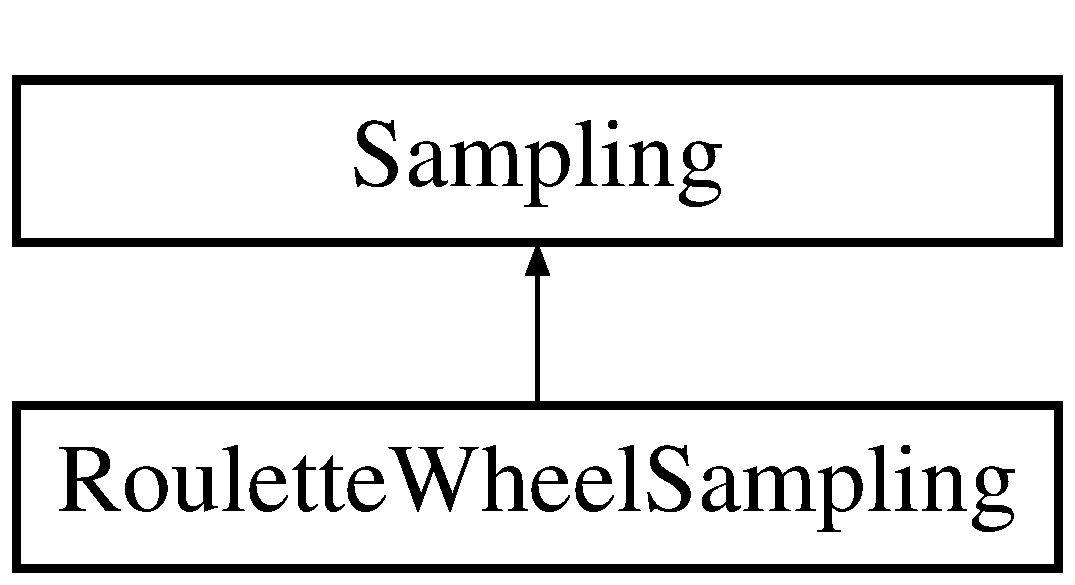
\includegraphics[height=2.000000cm]{classRouletteWheelSampling}
\end{center}
\end{figure}
\subsection*{Public Member Functions}
\begin{DoxyCompactItemize}
\item 
\hypertarget{classRouletteWheelSampling_ae9f93de1a052e204198887e0a47a5a1c}{\hyperlink{classRouletteWheelSampling_ae9f93de1a052e204198887e0a47a5a1c}{Roulette\-Wheel\-Sampling} ()}\label{classRouletteWheelSampling_ae9f93de1a052e204198887e0a47a5a1c}

\begin{DoxyCompactList}\small\item\em Default Constructor. \end{DoxyCompactList}\item 
std\-::vector$<$ \hyperlink{classParticle}{Particle} $>$ \hyperlink{classRouletteWheelSampling_ad9634cbe5aa5b112c823d252a1497313}{resample} (std\-::vector$<$ \hyperlink{classParticle}{Particle} $>$ particles, int number\-\_\-of\-\_\-particles, nav\-\_\-msgs\-::\-Occupancy\-Grid map)
\end{DoxyCompactItemize}
\subsection*{Additional Inherited Members}


\subsection{Detailed Description}
Roulette wheel implementation of sampling strategy pattern for particles. 

\subsection{Member Function Documentation}
\hypertarget{classRouletteWheelSampling_ad9634cbe5aa5b112c823d252a1497313}{\index{Roulette\-Wheel\-Sampling@{Roulette\-Wheel\-Sampling}!resample@{resample}}
\index{resample@{resample}!RouletteWheelSampling@{Roulette\-Wheel\-Sampling}}
\subsubsection[{resample}]{\setlength{\rightskip}{0pt plus 5cm}std\-::vector$<${\bf Particle}$>$ Roulette\-Wheel\-Sampling\-::resample (
\begin{DoxyParamCaption}
\item[{std\-::vector$<$ {\bf Particle} $>$}]{particles, }
\item[{int}]{number\-\_\-of\-\_\-particles, }
\item[{nav\-\_\-msgs\-::\-Occupancy\-Grid}]{map}
\end{DoxyParamCaption}
)\hspace{0.3cm}{\ttfamily [virtual]}}}\label{classRouletteWheelSampling_ad9634cbe5aa5b112c823d252a1497313}
Resampling according to strategy. 
\begin{DoxyParams}{Parameters}
{\em particles} & initial vector of particles. \\
\hline
{\em number\-\_\-of\-\_\-particles} & number of output particles. \\
\hline
{\em map} & map where particles should be sampled. \\
\hline
\end{DoxyParams}
\begin{DoxyReturn}{Returns}
output resampled particles. 
\end{DoxyReturn}


Implements \hyperlink{classSampling_ae9a5648926dda0a5d5ed4b55b9d96436}{Sampling}.



The documentation for this class was generated from the following file\-:\begin{DoxyCompactItemize}
\item 
include/localization/sampling\-\_\-strategies/\hyperlink{roulette__wheel__sampling_8h}{roulette\-\_\-wheel\-\_\-sampling.\-h}\end{DoxyCompactItemize}

\hypertarget{classSampling}{\section{Sampling Class Reference}
\label{classSampling}\index{Sampling@{Sampling}}
}


Abstract class for implementing the sampling strategy pattern.  




{\ttfamily \#include $<$sampling.\-h$>$}

Inheritance diagram for Sampling\-:\begin{figure}[H]
\begin{center}
\leavevmode
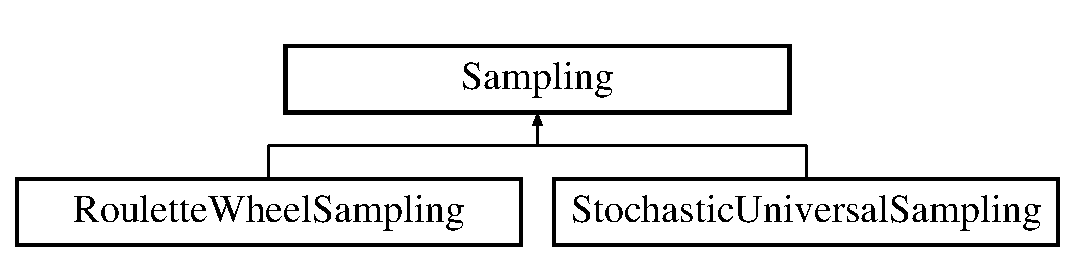
\includegraphics[height=2.000000cm]{classSampling}
\end{center}
\end{figure}
\subsection*{Public Member Functions}
\begin{DoxyCompactItemize}
\item 
virtual std\-::vector$<$ \hyperlink{classParticle}{Particle} $>$ \hyperlink{classSampling_ae9a5648926dda0a5d5ed4b55b9d96436}{resample} (std\-::vector$<$ \hyperlink{classParticle}{Particle} $>$ particles, int number\-\_\-of\-\_\-particles, nav\-\_\-msgs\-::\-Occupancy\-Grid map)=0
\begin{DoxyCompactList}\small\item\em Virtual Deconstructor. \end{DoxyCompactList}\item 
std\-::string \hyperlink{classSampling_ac355e000a52390164b1aaef3bdb384d2}{get\-\_\-name} ()
\item 
\hyperlink{classParticle}{Particle} \hyperlink{classSampling_acc4b8eb8fb757ee597b11594ce04f875}{random\-\_\-sample} (nav\-\_\-msgs\-::\-Occupancy\-Grid map)
\item 
std\-::vector$<$ \hyperlink{classParticle}{Particle} $>$ \hyperlink{classSampling_ae6b476b809237740fa413849caf6cab4}{renormalize} (std\-::vector$<$ \hyperlink{classParticle}{Particle} $>$ vector)
\end{DoxyCompactItemize}
\subsection*{Protected Attributes}
\begin{DoxyCompactItemize}
\item 
\hypertarget{classSampling_a42167134f19c2ad42aa796538356a7f8}{std\-::string \hyperlink{classSampling_a42167134f19c2ad42aa796538356a7f8}{\-\_\-name}}\label{classSampling_a42167134f19c2ad42aa796538356a7f8}

\begin{DoxyCompactList}\small\item\em sampling algorithm name. \end{DoxyCompactList}\item 
\hypertarget{classSampling_a77715cbe9a03102aa672fd34c776f042}{std\-::random\-\_\-device \hyperlink{classSampling_a77715cbe9a03102aa672fd34c776f042}{rd}}\label{classSampling_a77715cbe9a03102aa672fd34c776f042}

\begin{DoxyCompactList}\small\item\em random device. \end{DoxyCompactList}\item 
\hypertarget{classSampling_a696ac24b511359adaf2298c19b0d5883}{std\-::mt19937 \hyperlink{classSampling_a696ac24b511359adaf2298c19b0d5883}{\-\_\-gen}}\label{classSampling_a696ac24b511359adaf2298c19b0d5883}

\begin{DoxyCompactList}\small\item\em random number generator. \end{DoxyCompactList}\item 
\hypertarget{classSampling_a7dbb70549c2a72232358578f82173af7}{std\-::uniform\-\_\-real\-\_\-distribution\\*
$<$ double $>$ \hyperlink{classSampling_a7dbb70549c2a72232358578f82173af7}{\-\_\-distribution}}\label{classSampling_a7dbb70549c2a72232358578f82173af7}

\begin{DoxyCompactList}\small\item\em uniform distribution generator between 0 and 1. \end{DoxyCompactList}\end{DoxyCompactItemize}


\subsection{Detailed Description}
Abstract class for implementing the sampling strategy pattern. 

\subsection{Member Function Documentation}
\hypertarget{classSampling_ac355e000a52390164b1aaef3bdb384d2}{\index{Sampling@{Sampling}!get\-\_\-name@{get\-\_\-name}}
\index{get\-\_\-name@{get\-\_\-name}!Sampling@{Sampling}}
\subsubsection[{get\-\_\-name}]{\setlength{\rightskip}{0pt plus 5cm}std\-::string Sampling\-::get\-\_\-name (
\begin{DoxyParamCaption}
{}
\end{DoxyParamCaption}
)}}\label{classSampling_ac355e000a52390164b1aaef3bdb384d2}
Get sampling algorihtm name. \begin{DoxyReturn}{Returns}
output set of particles. 
\end{DoxyReturn}
\hypertarget{classSampling_acc4b8eb8fb757ee597b11594ce04f875}{\index{Sampling@{Sampling}!random\-\_\-sample@{random\-\_\-sample}}
\index{random\-\_\-sample@{random\-\_\-sample}!Sampling@{Sampling}}
\subsubsection[{random\-\_\-sample}]{\setlength{\rightskip}{0pt plus 5cm}{\bf Particle} Sampling\-::random\-\_\-sample (
\begin{DoxyParamCaption}
\item[{nav\-\_\-msgs\-::\-Occupancy\-Grid}]{map}
\end{DoxyParamCaption}
)}}\label{classSampling_acc4b8eb8fb757ee597b11594ce04f875}
Get random particle from map 
\begin{DoxyParams}{Parameters}
{\em map} & map where particles should be sampled. \\
\hline
\end{DoxyParams}
\begin{DoxyReturn}{Returns}

\end{DoxyReturn}
\hypertarget{classSampling_ae6b476b809237740fa413849caf6cab4}{\index{Sampling@{Sampling}!renormalize@{renormalize}}
\index{renormalize@{renormalize}!Sampling@{Sampling}}
\subsubsection[{renormalize}]{\setlength{\rightskip}{0pt plus 5cm}std\-::vector$<${\bf Particle}$>$ Sampling\-::renormalize (
\begin{DoxyParamCaption}
\item[{std\-::vector$<$ {\bf Particle} $>$}]{vector}
\end{DoxyParamCaption}
)}}\label{classSampling_ae6b476b809237740fa413849caf6cab4}
Renormalize a vector of particles so sum(weights)=1 
\begin{DoxyParams}{Parameters}
{\em vector} & vector of particles. \\
\hline
\end{DoxyParams}
\begin{DoxyReturn}{Returns}
renormalized vector of particles . 
\end{DoxyReturn}
\hypertarget{classSampling_ae9a5648926dda0a5d5ed4b55b9d96436}{\index{Sampling@{Sampling}!resample@{resample}}
\index{resample@{resample}!Sampling@{Sampling}}
\subsubsection[{resample}]{\setlength{\rightskip}{0pt plus 5cm}virtual std\-::vector$<${\bf Particle}$>$ Sampling\-::resample (
\begin{DoxyParamCaption}
\item[{std\-::vector$<$ {\bf Particle} $>$}]{particles, }
\item[{int}]{number\-\_\-of\-\_\-particles, }
\item[{nav\-\_\-msgs\-::\-Occupancy\-Grid}]{map}
\end{DoxyParamCaption}
)\hspace{0.3cm}{\ttfamily [pure virtual]}}}\label{classSampling_ae9a5648926dda0a5d5ed4b55b9d96436}


Virtual Deconstructor. 

Resampling according to strategy. 
\begin{DoxyParams}{Parameters}
{\em particles} & initial vector of particles. \\
\hline
{\em number\-\_\-of\-\_\-particles} & number of output particles. \\
\hline
{\em map} & map where particles should be sampled. \\
\hline
\end{DoxyParams}
\begin{DoxyReturn}{Returns}
output resampled particles. 
\end{DoxyReturn}


Implemented in \hyperlink{classRouletteWheelSampling_ad9634cbe5aa5b112c823d252a1497313}{Roulette\-Wheel\-Sampling}, and \hyperlink{classStochasticUniversalSampling_aa46ab5185de58679355e388eb3e05d6d}{Stochastic\-Universal\-Sampling}.



The documentation for this class was generated from the following file\-:\begin{DoxyCompactItemize}
\item 
include/localization/sampling\-\_\-strategies/\hyperlink{sampling_8h}{sampling.\-h}\end{DoxyCompactItemize}

\hypertarget{classSamplingParser}{\section{Sampling\-Parser Class Reference}
\label{classSamplingParser}\index{Sampling\-Parser@{Sampling\-Parser}}
}


Class that parses from the rosparam server the sampling strategy to be used.  




{\ttfamily \#include $<$sampling\-\_\-parser.\-h$>$}

\subsection*{Public Member Functions}
\begin{DoxyCompactItemize}
\item 
\hypertarget{classSamplingParser_a753d77bb855ace7e0b4ef98b59e4721a}{\hyperlink{classSamplingParser_a753d77bb855ace7e0b4ef98b59e4721a}{Sampling\-Parser} (ros\-::\-Node\-Handle nh)}\label{classSamplingParser_a753d77bb855ace7e0b4ef98b59e4721a}

\begin{DoxyCompactList}\small\item\em Default Constructor. \end{DoxyCompactList}\item 
\hypertarget{classSamplingParser_a7d7c0cdba71dbe81494cc409322150c3}{\hyperlink{classSamplingParser_a7d7c0cdba71dbe81494cc409322150c3}{$\sim$\-Sampling\-Parser} ()}\label{classSamplingParser_a7d7c0cdba71dbe81494cc409322150c3}

\begin{DoxyCompactList}\small\item\em Class Deconstructor. \end{DoxyCompactList}\item 
\hypertarget{classSamplingParser_ac9096129452828bd6fde815f68ce1d30}{\hyperlink{sampling_8h_adf4afed667a21b30f8ff816aae609bf7}{Sampling\-Ptr} \hyperlink{classSamplingParser_ac9096129452828bd6fde815f68ce1d30}{get\-\_\-sampling\-\_\-strategy} ()}\label{classSamplingParser_ac9096129452828bd6fde815f68ce1d30}

\begin{DoxyCompactList}\small\item\em Get parsed sampling strategy implementation. \end{DoxyCompactList}\end{DoxyCompactItemize}


\subsection{Detailed Description}
Class that parses from the rosparam server the sampling strategy to be used. 

The documentation for this class was generated from the following file\-:\begin{DoxyCompactItemize}
\item 
include/localization/parsers/\hyperlink{sampling__parser_8h}{sampling\-\_\-parser.\-h}\end{DoxyCompactItemize}

\hypertarget{classSensorUpdate}{\section{Sensor\-Update Class Reference}
\label{classSensorUpdate}\index{Sensor\-Update@{Sensor\-Update}}
}


Abstract class for implementing the sensor update strategy pattern.  




{\ttfamily \#include $<$sensor\-\_\-update.\-h$>$}

Inheritance diagram for Sensor\-Update\-:\begin{figure}[H]
\begin{center}
\leavevmode
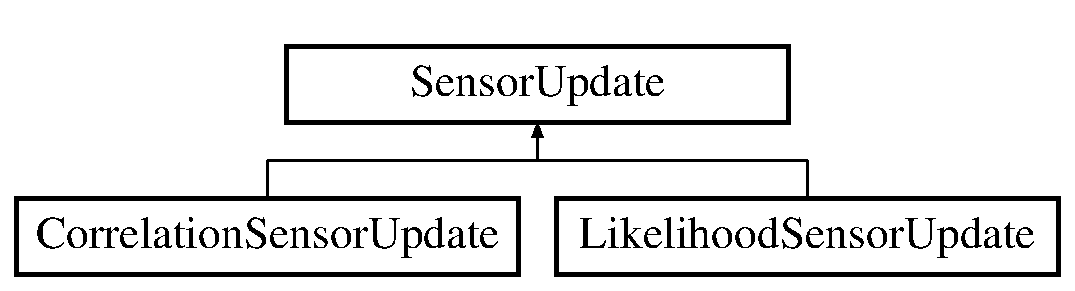
\includegraphics[height=2.000000cm]{classSensorUpdate}
\end{center}
\end{figure}
\subsection*{Public Member Functions}
\begin{DoxyCompactItemize}
\item 
virtual double \hyperlink{classSensorUpdate_a9bd0792d09b9425b854c6220b6712a52}{a\-\_\-posteriori} (double a\-\_\-priori, \hyperlink{occupancy__map_8h_aea86d1b633e7d9b44b660a39fa9b50f7}{Occupancy\-Map\-Ptr} a\-\_\-priori\-\_\-map, geometry\-\_\-msgs\-::\-Pose\-With\-Covariance\-Stamped pose, const sensor\-\_\-msgs\-::\-Laser\-Scan\-::\-Const\-Ptr \&msg)=0
\begin{DoxyCompactList}\small\item\em Virtual Deconstructor. \end{DoxyCompactList}\item 
void \hyperlink{classSensorUpdate_a01586f280eb8dbad45283696f3301221}{set\-\_\-map} (const nav\-\_\-msgs\-::\-Occupancy\-Grid\-::\-Const\-Ptr \&map)
\item 
std\-::string \hyperlink{classSensorUpdate_a0686226d99e3578bce52920fcb46577b}{get\-\_\-name} ()
\item 
std\-::string \hyperlink{classSensorUpdate_aa7b11255fd04d98eae6d265de84552df}{get\-\_\-reference\-\_\-frame} ()
\end{DoxyCompactItemize}
\subsection*{Protected Attributes}
\begin{DoxyCompactItemize}
\item 
\hypertarget{classSensorUpdate_a7e999f7c8092407e8df50c533cc50d72}{std\-::string \hyperlink{classSensorUpdate_a7e999f7c8092407e8df50c533cc50d72}{\-\_\-name}}\label{classSensorUpdate_a7e999f7c8092407e8df50c533cc50d72}

\begin{DoxyCompactList}\small\item\em algorithm name. \end{DoxyCompactList}\item 
\hypertarget{classSensorUpdate_a1b19df70d6264e226ace9ce4634fb9fa}{\hyperlink{classOccupancyMap}{Occupancy\-Map} \hyperlink{classSensorUpdate_a1b19df70d6264e226ace9ce4634fb9fa}{\-\_\-map}}\label{classSensorUpdate_a1b19df70d6264e226ace9ce4634fb9fa}

\begin{DoxyCompactList}\small\item\em global map. \end{DoxyCompactList}\end{DoxyCompactItemize}


\subsection{Detailed Description}
Abstract class for implementing the sensor update strategy pattern. 

\subsection{Member Function Documentation}
\hypertarget{classSensorUpdate_a9bd0792d09b9425b854c6220b6712a52}{\index{Sensor\-Update@{Sensor\-Update}!a\-\_\-posteriori@{a\-\_\-posteriori}}
\index{a\-\_\-posteriori@{a\-\_\-posteriori}!SensorUpdate@{Sensor\-Update}}
\subsubsection[{a\-\_\-posteriori}]{\setlength{\rightskip}{0pt plus 5cm}virtual double Sensor\-Update\-::a\-\_\-posteriori (
\begin{DoxyParamCaption}
\item[{double}]{a\-\_\-priori, }
\item[{{\bf Occupancy\-Map\-Ptr}}]{a\-\_\-priori\-\_\-map, }
\item[{geometry\-\_\-msgs\-::\-Pose\-With\-Covariance\-Stamped}]{pose, }
\item[{const sensor\-\_\-msgs\-::\-Laser\-Scan\-::\-Const\-Ptr \&}]{msg}
\end{DoxyParamCaption}
)\hspace{0.3cm}{\ttfamily [pure virtual]}}}\label{classSensorUpdate_a9bd0792d09b9425b854c6220b6712a52}


Virtual Deconstructor. 

Get a posteriori probability of being in a pose given the msg. 
\begin{DoxyParams}{Parameters}
{\em a\-\_\-priori} & a priori probability of being in a pose. \\
\hline
{\em a\-\_\-priori\-\_\-map} & a priori pointer to believed map. \\
\hline
{\em pose} & believed pose. \\
\hline
{\em msg} & recieved scan msg. \\
\hline
\end{DoxyParams}
\begin{DoxyReturn}{Returns}
a posteriori probability 
\end{DoxyReturn}


Implemented in \hyperlink{classLikelihoodSensorUpdate_aa7a4eaae56fb86af98f428b598f46962}{Likelihood\-Sensor\-Update}, and \hyperlink{classCorrelationSensorUpdate_a72b2bd8daa21b7c76de0eb306e579906}{Correlation\-Sensor\-Update}.

\hypertarget{classSensorUpdate_a0686226d99e3578bce52920fcb46577b}{\index{Sensor\-Update@{Sensor\-Update}!get\-\_\-name@{get\-\_\-name}}
\index{get\-\_\-name@{get\-\_\-name}!SensorUpdate@{Sensor\-Update}}
\subsubsection[{get\-\_\-name}]{\setlength{\rightskip}{0pt plus 5cm}std\-::string Sensor\-Update\-::get\-\_\-name (
\begin{DoxyParamCaption}
{}
\end{DoxyParamCaption}
)}}\label{classSensorUpdate_a0686226d99e3578bce52920fcb46577b}
Get algorithm name. \begin{DoxyReturn}{Returns}

\end{DoxyReturn}
\hypertarget{classSensorUpdate_aa7b11255fd04d98eae6d265de84552df}{\index{Sensor\-Update@{Sensor\-Update}!get\-\_\-reference\-\_\-frame@{get\-\_\-reference\-\_\-frame}}
\index{get\-\_\-reference\-\_\-frame@{get\-\_\-reference\-\_\-frame}!SensorUpdate@{Sensor\-Update}}
\subsubsection[{get\-\_\-reference\-\_\-frame}]{\setlength{\rightskip}{0pt plus 5cm}std\-::string Sensor\-Update\-::get\-\_\-reference\-\_\-frame (
\begin{DoxyParamCaption}
{}
\end{DoxyParamCaption}
)}}\label{classSensorUpdate_aa7b11255fd04d98eae6d265de84552df}
Get reference frame of update step. \begin{DoxyReturn}{Returns}

\end{DoxyReturn}
\hypertarget{classSensorUpdate_a01586f280eb8dbad45283696f3301221}{\index{Sensor\-Update@{Sensor\-Update}!set\-\_\-map@{set\-\_\-map}}
\index{set\-\_\-map@{set\-\_\-map}!SensorUpdate@{Sensor\-Update}}
\subsubsection[{set\-\_\-map}]{\setlength{\rightskip}{0pt plus 5cm}void Sensor\-Update\-::set\-\_\-map (
\begin{DoxyParamCaption}
\item[{const nav\-\_\-msgs\-::\-Occupancy\-Grid\-::\-Const\-Ptr \&}]{map}
\end{DoxyParamCaption}
)}}\label{classSensorUpdate_a01586f280eb8dbad45283696f3301221}
Set global map to the update algorithm. 
\begin{DoxyParams}{Parameters}
{\em map} & Occupancy grid msg pointer. \\
\hline
\end{DoxyParams}


The documentation for this class was generated from the following file\-:\begin{DoxyCompactItemize}
\item 
include/localization/sensor\-\_\-update\-\_\-strategies/\hyperlink{sensor__update_8h}{sensor\-\_\-update.\-h}\end{DoxyCompactItemize}

\hypertarget{classSensorUpdateParser}{\section{Sensor\-Update\-Parser Class Reference}
\label{classSensorUpdateParser}\index{Sensor\-Update\-Parser@{Sensor\-Update\-Parser}}
}


Class that parses from the rosparam server the sensor update strategy to be used.  




{\ttfamily \#include $<$sensor\-\_\-update\-\_\-parser.\-h$>$}

\subsection*{Public Member Functions}
\begin{DoxyCompactItemize}
\item 
\hypertarget{classSensorUpdateParser_a75485f13f3fc802a94c5246c05367e7b}{\hyperlink{classSensorUpdateParser_a75485f13f3fc802a94c5246c05367e7b}{Sensor\-Update\-Parser} (ros\-::\-Node\-Handle nh)}\label{classSensorUpdateParser_a75485f13f3fc802a94c5246c05367e7b}

\begin{DoxyCompactList}\small\item\em Default Constructor. \end{DoxyCompactList}\item 
\hypertarget{classSensorUpdateParser_a8da82b578ce394108d4fef03ef8bbd6c}{\hyperlink{classSensorUpdateParser_a8da82b578ce394108d4fef03ef8bbd6c}{$\sim$\-Sensor\-Update\-Parser} ()}\label{classSensorUpdateParser_a8da82b578ce394108d4fef03ef8bbd6c}

\begin{DoxyCompactList}\small\item\em Class Deconstructor. \end{DoxyCompactList}\item 
\hypertarget{classSensorUpdateParser_a5513b406355330377c64825c30264e44}{\hyperlink{sensor__update_8h_a7bfe6ec1a05f2f99b0974d5cbd8b8b7b}{Sensor\-Update\-Ptr} \hyperlink{classSensorUpdateParser_a5513b406355330377c64825c30264e44}{get\-\_\-sensor\-\_\-update} ()}\label{classSensorUpdateParser_a5513b406355330377c64825c30264e44}

\begin{DoxyCompactList}\small\item\em Get parsed sensor strategy implementation. \end{DoxyCompactList}\end{DoxyCompactItemize}


\subsection{Detailed Description}
Class that parses from the rosparam server the sensor update strategy to be used. 

The documentation for this class was generated from the following file\-:\begin{DoxyCompactItemize}
\item 
include/localization/parsers/\hyperlink{sensor__update__parser_8h}{sensor\-\_\-update\-\_\-parser.\-h}\end{DoxyCompactItemize}

\hypertarget{classStochasticUniversalSampling}{\section{Stochastic\-Universal\-Sampling Class Reference}
\label{classStochasticUniversalSampling}\index{Stochastic\-Universal\-Sampling@{Stochastic\-Universal\-Sampling}}
}


Stochastic universal implementation of sampling strategy pattern for particles.  




{\ttfamily \#include $<$stochastic\-\_\-universal\-\_\-sampling.\-h$>$}

Inheritance diagram for Stochastic\-Universal\-Sampling\-:\begin{figure}[H]
\begin{center}
\leavevmode
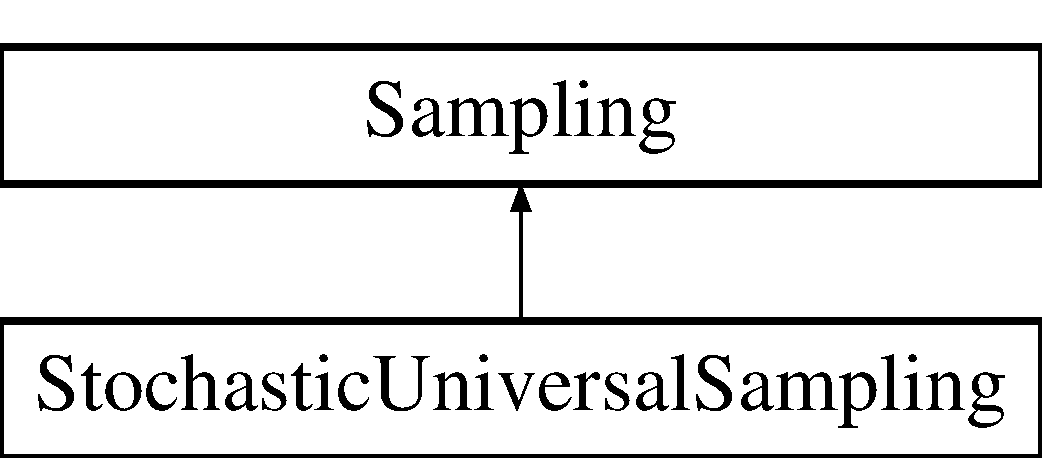
\includegraphics[height=2.000000cm]{classStochasticUniversalSampling}
\end{center}
\end{figure}
\subsection*{Public Member Functions}
\begin{DoxyCompactItemize}
\item 
\hypertarget{classStochasticUniversalSampling_ac6d8388314fb9eec1341b6879eec4cca}{\hyperlink{classStochasticUniversalSampling_ac6d8388314fb9eec1341b6879eec4cca}{Stochastic\-Universal\-Sampling} ()}\label{classStochasticUniversalSampling_ac6d8388314fb9eec1341b6879eec4cca}

\begin{DoxyCompactList}\small\item\em Default Constructor. \end{DoxyCompactList}\item 
std\-::vector$<$ \hyperlink{classParticle}{Particle} $>$ \hyperlink{classStochasticUniversalSampling_aa46ab5185de58679355e388eb3e05d6d}{resample} (std\-::vector$<$ \hyperlink{classParticle}{Particle} $>$ particles, int number\-\_\-of\-\_\-particles, nav\-\_\-msgs\-::\-Occupancy\-Grid map)
\end{DoxyCompactItemize}
\subsection*{Additional Inherited Members}


\subsection{Detailed Description}
Stochastic universal implementation of sampling strategy pattern for particles. 

\subsection{Member Function Documentation}
\hypertarget{classStochasticUniversalSampling_aa46ab5185de58679355e388eb3e05d6d}{\index{Stochastic\-Universal\-Sampling@{Stochastic\-Universal\-Sampling}!resample@{resample}}
\index{resample@{resample}!StochasticUniversalSampling@{Stochastic\-Universal\-Sampling}}
\subsubsection[{resample}]{\setlength{\rightskip}{0pt plus 5cm}std\-::vector$<${\bf Particle}$>$ Stochastic\-Universal\-Sampling\-::resample (
\begin{DoxyParamCaption}
\item[{std\-::vector$<$ {\bf Particle} $>$}]{particles, }
\item[{int}]{number\-\_\-of\-\_\-particles, }
\item[{nav\-\_\-msgs\-::\-Occupancy\-Grid}]{map}
\end{DoxyParamCaption}
)\hspace{0.3cm}{\ttfamily [virtual]}}}\label{classStochasticUniversalSampling_aa46ab5185de58679355e388eb3e05d6d}
Resampling according to strategy. 
\begin{DoxyParams}{Parameters}
{\em particles} & initial vector of particles. \\
\hline
{\em number\-\_\-of\-\_\-particles} & number of output particles. \\
\hline
{\em map} & map where particles should be sampled. \\
\hline
\end{DoxyParams}
\begin{DoxyReturn}{Returns}
output resampled particles. 
\end{DoxyReturn}


Implements \hyperlink{classSampling_ae9a5648926dda0a5d5ed4b55b9d96436}{Sampling}.



The documentation for this class was generated from the following file\-:\begin{DoxyCompactItemize}
\item 
include/localization/sampling\-\_\-strategies/\hyperlink{stochastic__universal__sampling_8h}{stochastic\-\_\-universal\-\_\-sampling.\-h}\end{DoxyCompactItemize}

\hypertarget{classVelocityMotionUpdate}{\section{Velocity\-Motion\-Update Class Reference}
\label{classVelocityMotionUpdate}\index{Velocity\-Motion\-Update@{Velocity\-Motion\-Update}}
}


Velocity model implementation of motion update algorithm.  




{\ttfamily \#include $<$velocity\-\_\-motion\-\_\-update.\-h$>$}

Inheritance diagram for Velocity\-Motion\-Update\-:\begin{figure}[H]
\begin{center}
\leavevmode
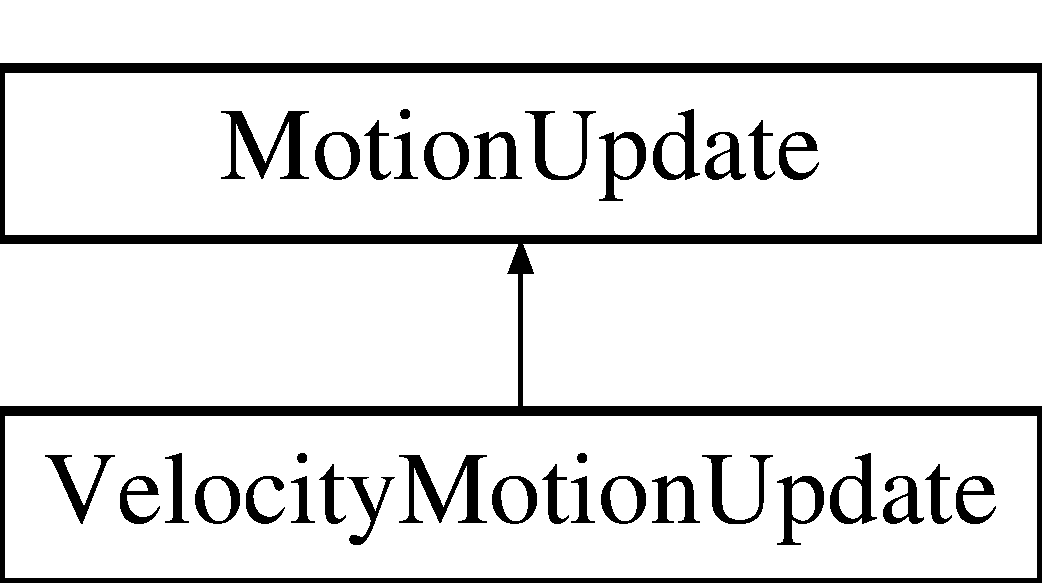
\includegraphics[height=2.000000cm]{classVelocityMotionUpdate}
\end{center}
\end{figure}
\subsection*{Public Member Functions}
\begin{DoxyCompactItemize}
\item 
\hypertarget{classVelocityMotionUpdate_a7a9a88ec65e09028cdcfd2c821b4c1bd}{\hyperlink{classVelocityMotionUpdate_a7a9a88ec65e09028cdcfd2c821b4c1bd}{Velocity\-Motion\-Update} ()}\label{classVelocityMotionUpdate_a7a9a88ec65e09028cdcfd2c821b4c1bd}

\begin{DoxyCompactList}\small\item\em Default Constructor. \end{DoxyCompactList}\item 
geometry\-\_\-msgs\-::\-Pose\-With\-Covariance\-Stamped \hyperlink{classVelocityMotionUpdate_a1b532d900fd3393e70f7a70f153c3e08}{predict} (geometry\-\_\-msgs\-::\-Pose\-With\-Covariance\-Stamped pose, const nav\-\_\-msgs\-::\-Odometry\-::\-Const\-Ptr \&old\-\_\-msg, const nav\-\_\-msgs\-::\-Odometry\-::\-Const\-Ptr \&new\-\_\-msg)
\end{DoxyCompactItemize}
\subsection*{Additional Inherited Members}


\subsection{Detailed Description}
Velocity model implementation of motion update algorithm. 

\subsection{Member Function Documentation}
\hypertarget{classVelocityMotionUpdate_a1b532d900fd3393e70f7a70f153c3e08}{\index{Velocity\-Motion\-Update@{Velocity\-Motion\-Update}!predict@{predict}}
\index{predict@{predict}!VelocityMotionUpdate@{Velocity\-Motion\-Update}}
\subsubsection[{predict}]{\setlength{\rightskip}{0pt plus 5cm}geometry\-\_\-msgs\-::\-Pose\-With\-Covariance\-Stamped Velocity\-Motion\-Update\-::predict (
\begin{DoxyParamCaption}
\item[{geometry\-\_\-msgs\-::\-Pose\-With\-Covariance\-Stamped}]{pose, }
\item[{const nav\-\_\-msgs\-::\-Odometry\-::\-Const\-Ptr \&}]{old\-\_\-msg, }
\item[{const nav\-\_\-msgs\-::\-Odometry\-::\-Const\-Ptr \&}]{new\-\_\-msg}
\end{DoxyParamCaption}
)\hspace{0.3cm}{\ttfamily [virtual]}}}\label{classVelocityMotionUpdate_a1b532d900fd3393e70f7a70f153c3e08}
Predict the new pose. 
\begin{DoxyParams}{Parameters}
{\em pose} & current pose. \\
\hline
{\em old\-\_\-msg} & last odometry msg. \\
\hline
{\em new\-\_\-msg} & new odometry msg. \\
\hline
\end{DoxyParams}
\begin{DoxyReturn}{Returns}

\end{DoxyReturn}


Implements \hyperlink{classMotionUpdate_a86e028d43981218ddf6e354e8f201e75}{Motion\-Update}.



The documentation for this class was generated from the following file\-:\begin{DoxyCompactItemize}
\item 
include/localization/motion\-\_\-update\-\_\-strategies/\hyperlink{velocity__motion__update_8h}{velocity\-\_\-motion\-\_\-update.\-h}\end{DoxyCompactItemize}

\chapter{File Documentation}
\hypertarget{localization__behaviour_8h}{\section{include/localization/behaviour/localization\-\_\-behaviour.h File Reference}
\label{localization__behaviour_8h}\index{include/localization/behaviour/localization\-\_\-behaviour.\-h@{include/localization/behaviour/localization\-\_\-behaviour.\-h}}
}
{\ttfamily \#include $<$ros/ros.\-h$>$}\\*
{\ttfamily \#include \char`\"{}localization/filtering\-\_\-strategies/particle\-\_\-filter.\-h\char`\"{}}\\*
{\ttfamily \#include \char`\"{}localization/util/particle.\-h\char`\"{}}\\*
{\ttfamily \#include $<$sensor\-\_\-msgs/\-Laser\-Scan.\-h$>$}\\*
{\ttfamily \#include $<$nav\-\_\-msgs/\-Odometry.\-h$>$}\\*
{\ttfamily \#include $<$nav\-\_\-msgs/\-Occupancy\-Grid.\-h$>$}\\*
{\ttfamily \#include $<$geometry\-\_\-msgs/\-Pose\-Array.\-h$>$}\\*
{\ttfamily \#include $<$tf/transform\-\_\-broadcaster.\-h$>$}\\*
\subsection*{Classes}
\begin{DoxyCompactItemize}
\item 
class \hyperlink{classLocalizationBehaviour}{Localization\-Behaviour}
\begin{DoxyCompactList}\small\item\em Class that sequences the pose filter algorithm from ros msgs and publishes the result. \end{DoxyCompactList}\end{DoxyCompactItemize}


\subsection{Detailed Description}
\begin{DoxyDate}{Date}
Dec 4, 2015 
\end{DoxyDate}
\begin{DoxyAuthor}{Author}
Sebastian Curi 
\end{DoxyAuthor}
\begin{DoxyRefDesc}{Bug}
\item[\hyperlink{bug__bug000001}{Bug}]No known bug. \end{DoxyRefDesc}

\hypertarget{particle__filter_8h}{\section{include/localization/filtering\-\_\-strategies/particle\-\_\-filter.h File Reference}
\label{particle__filter_8h}\index{include/localization/filtering\-\_\-strategies/particle\-\_\-filter.\-h@{include/localization/filtering\-\_\-strategies/particle\-\_\-filter.\-h}}
}
{\ttfamily \#include \char`\"{}localization/util/particle.\-h\char`\"{}}\\*
{\ttfamily \#include \char`\"{}localization/filtering\-\_\-strategies/pose\-\_\-filter.\-h\char`\"{}}\\*
\subsection*{Classes}
\begin{DoxyCompactItemize}
\item 
class \hyperlink{classParticleFilter}{Particle\-Filter}
\begin{DoxyCompactList}\small\item\em Implementation of the particle filter algorithm. \end{DoxyCompactList}\end{DoxyCompactItemize}


\subsection{Detailed Description}
\begin{DoxyDate}{Date}
Dec 4, 2015 
\end{DoxyDate}
\begin{DoxyAuthor}{Author}
Sebastian Curi 
\end{DoxyAuthor}
\begin{DoxyRefDesc}{Bug}
\item[\hyperlink{bug__bug000002}{Bug}]No known bug. \end{DoxyRefDesc}

\hypertarget{pose__filter_8h}{\section{include/localization/filtering\-\_\-strategies/pose\-\_\-filter.h File Reference}
\label{pose__filter_8h}\index{include/localization/filtering\-\_\-strategies/pose\-\_\-filter.\-h@{include/localization/filtering\-\_\-strategies/pose\-\_\-filter.\-h}}
}
{\ttfamily \#include $<$sensor\-\_\-msgs/\-Laser\-Scan.\-h$>$}\\*
{\ttfamily \#include $<$nav\-\_\-msgs/\-Odometry.\-h$>$}\\*
{\ttfamily \#include $<$geometry\-\_\-msgs/\-Pose\-With\-Covariance\-Stamped.\-h$>$}\\*
{\ttfamily \#include $<$string$>$}\\*
{\ttfamily \#include \char`\"{}localization/sensor\-\_\-update\-\_\-strategies/sensor\-\_\-update.\-h\char`\"{}}\\*
{\ttfamily \#include \char`\"{}localization/motion\-\_\-update\-\_\-strategies/motion\-\_\-update.\-h\char`\"{}}\\*
{\ttfamily \#include \char`\"{}localization/sampling\-\_\-strategies/sampling.\-h\char`\"{}}\\*
{\ttfamily \#include \char`\"{}pose\-\_\-filter.\-hpp\char`\"{}}\\*
\subsection*{Classes}
\begin{DoxyCompactItemize}
\item 
class \hyperlink{classPoseFilter}{Pose\-Filter}
\begin{DoxyCompactList}\small\item\em Abstract class for implementing the pose filter strategy pattern. \end{DoxyCompactList}\end{DoxyCompactItemize}
\subsection*{Typedefs}
\begin{DoxyCompactItemize}
\item 
\hypertarget{pose__filter_8h_a9df59d7c2f322f00bdd8eccab6d3fd73}{typedef boost\-::shared\-\_\-ptr\\*
$<$ \hyperlink{classPoseFilter}{Pose\-Filter} $>$ \hyperlink{pose__filter_8h_a9df59d7c2f322f00bdd8eccab6d3fd73}{Pose\-Filter\-Ptr}}\label{pose__filter_8h_a9df59d7c2f322f00bdd8eccab6d3fd73}

\begin{DoxyCompactList}\small\item\em Shared pointer to Pose filter class. \end{DoxyCompactList}\end{DoxyCompactItemize}


\subsection{Detailed Description}
This is an abstract class for implementing a localization filter algorithm using a strategy pattern.

\begin{DoxyDate}{Date}
Dec 4, 2015 
\end{DoxyDate}
\begin{DoxyAuthor}{Author}
Sebastian Curi 
\end{DoxyAuthor}
\begin{DoxyRefDesc}{Bug}
\item[\hyperlink{bug__bug000003}{Bug}]No known bug. \end{DoxyRefDesc}

\hypertarget{pose__filter_8hpp}{\section{include/localization/filtering\-\_\-strategies/pose\-\_\-filter.hpp File Reference}
\label{pose__filter_8hpp}\index{include/localization/filtering\-\_\-strategies/pose\-\_\-filter.\-hpp@{include/localization/filtering\-\_\-strategies/pose\-\_\-filter.\-hpp}}
}


\subsection{Detailed Description}
\begin{DoxyDate}{Date}
Dec 5, 2015 
\end{DoxyDate}
\begin{DoxyAuthor}{Author}
Sebastian Curi 
\end{DoxyAuthor}
\begin{DoxyRefDesc}{Bug}
\item[\hyperlink{bug__bug000004}{Bug}]No known bugs. \end{DoxyRefDesc}

\hypertarget{motion__update_8h}{\section{include/localization/motion\-\_\-update\-\_\-strategies/motion\-\_\-update.h File Reference}
\label{motion__update_8h}\index{include/localization/motion\-\_\-update\-\_\-strategies/motion\-\_\-update.\-h@{include/localization/motion\-\_\-update\-\_\-strategies/motion\-\_\-update.\-h}}
}
{\ttfamily \#include $<$tf/transform\-\_\-datatypes.\-h$>$}\\*
{\ttfamily \#include $<$nav\-\_\-msgs/\-Odometry.\-h$>$}\\*
{\ttfamily \#include $<$geometry\-\_\-msgs/\-Pose\-With\-Covariance\-Stamped.\-h$>$}\\*
\subsection*{Classes}
\begin{DoxyCompactItemize}
\item 
class \hyperlink{classMotionUpdate}{Motion\-Update}
\begin{DoxyCompactList}\small\item\em Abstract class for implementing the motion update strategy pattern. \end{DoxyCompactList}\end{DoxyCompactItemize}
\subsection*{Typedefs}
\begin{DoxyCompactItemize}
\item 
\hypertarget{motion__update_8h_aec1cf0d54c70c4dacac639ab488bf948}{typedef boost\-::shared\-\_\-ptr\\*
$<$ \hyperlink{classMotionUpdate}{Motion\-Update} $>$ \hyperlink{motion__update_8h_aec1cf0d54c70c4dacac639ab488bf948}{Motion\-Update\-Ptr}}\label{motion__update_8h_aec1cf0d54c70c4dacac639ab488bf948}

\begin{DoxyCompactList}\small\item\em Shared pointer to motion\-\_\-update class. \end{DoxyCompactList}\end{DoxyCompactItemize}


\subsection{Detailed Description}
\begin{DoxyDate}{Date}
Dec 4, 2015 
\end{DoxyDate}
\begin{DoxyAuthor}{Author}
Sebastian Curi 
\end{DoxyAuthor}
\begin{DoxyRefDesc}{Bug}
\item[\hyperlink{bug__bug000005}{Bug}]No known bug. \end{DoxyRefDesc}

\hypertarget{odometry__motion__update_8h}{\section{include/localization/motion\-\_\-update\-\_\-strategies/odometry\-\_\-motion\-\_\-update.h File Reference}
\label{odometry__motion__update_8h}\index{include/localization/motion\-\_\-update\-\_\-strategies/odometry\-\_\-motion\-\_\-update.\-h@{include/localization/motion\-\_\-update\-\_\-strategies/odometry\-\_\-motion\-\_\-update.\-h}}
}
{\ttfamily \#include $<$localization/motion\-\_\-update\-\_\-strategies/motion\-\_\-update.\-h$>$}\\*
\subsection*{Classes}
\begin{DoxyCompactItemize}
\item 
class \hyperlink{classOdometryMotionUpdate}{Odometry\-Motion\-Update}
\begin{DoxyCompactList}\small\item\em Odometry model implementation of motion update algorithm. \end{DoxyCompactList}\end{DoxyCompactItemize}


\subsection{Detailed Description}
\begin{DoxyDate}{Date}
Dec 4, 2015 
\end{DoxyDate}
\begin{DoxyAuthor}{Author}
Sebastian Curi 
\end{DoxyAuthor}
\begin{DoxyRefDesc}{Bug}
\item[\hyperlink{bug__bug000006}{Bug}]No known bug. \end{DoxyRefDesc}

\hypertarget{velocity__motion__update_8h}{\section{include/localization/motion\-\_\-update\-\_\-strategies/velocity\-\_\-motion\-\_\-update.h File Reference}
\label{velocity__motion__update_8h}\index{include/localization/motion\-\_\-update\-\_\-strategies/velocity\-\_\-motion\-\_\-update.\-h@{include/localization/motion\-\_\-update\-\_\-strategies/velocity\-\_\-motion\-\_\-update.\-h}}
}
{\ttfamily \#include $<$localization/motion\-\_\-update\-\_\-strategies/motion\-\_\-update.\-h$>$}\\*
\subsection*{Classes}
\begin{DoxyCompactItemize}
\item 
class \hyperlink{classVelocityMotionUpdate}{Velocity\-Motion\-Update}
\begin{DoxyCompactList}\small\item\em Velocity model implementation of motion update algorithm. \end{DoxyCompactList}\end{DoxyCompactItemize}


\subsection{Detailed Description}
\begin{DoxyDate}{Date}
Dec 4, 2015 
\end{DoxyDate}
\begin{DoxyAuthor}{Author}
Sebastian Curi 
\end{DoxyAuthor}
\begin{DoxyRefDesc}{Bug}
\item[\hyperlink{bug__bug000007}{Bug}]No known bug. \end{DoxyRefDesc}

\hypertarget{filter__parser_8h}{\section{include/localization/parsers/filter\-\_\-parser.h File Reference}
\label{filter__parser_8h}\index{include/localization/parsers/filter\-\_\-parser.\-h@{include/localization/parsers/filter\-\_\-parser.\-h}}
}
{\ttfamily \#include $<$ros/ros.\-h$>$}\\*
{\ttfamily \#include \char`\"{}localization/filtering\-\_\-strategies/particle\-\_\-filter.\-h\char`\"{}}\\*
\subsection*{Classes}
\begin{DoxyCompactItemize}
\item 
class \hyperlink{classFilterParser}{Filter\-Parser}
\begin{DoxyCompactList}\small\item\em Class that parses from the rosparam server the ros strategy to be used. \end{DoxyCompactList}\end{DoxyCompactItemize}


\subsection{Detailed Description}
\begin{DoxyDate}{Date}
Dec 5, 2015 
\end{DoxyDate}
\begin{DoxyAuthor}{Author}
Sebastian Curi 
\end{DoxyAuthor}
\begin{DoxyRefDesc}{Bug}
\item[\hyperlink{bug__bug000008}{Bug}]No known bugs. \end{DoxyRefDesc}

\hypertarget{motion__update__parser_8h}{\section{include/localization/parsers/motion\-\_\-update\-\_\-parser.h File Reference}
\label{motion__update__parser_8h}\index{include/localization/parsers/motion\-\_\-update\-\_\-parser.\-h@{include/localization/parsers/motion\-\_\-update\-\_\-parser.\-h}}
}
{\ttfamily \#include $<$ros/ros.\-h$>$}\\*
{\ttfamily \#include \char`\"{}localization/motion\-\_\-update\-\_\-strategies/odometry\-\_\-motion\-\_\-update.\-h\char`\"{}}\\*
{\ttfamily \#include \char`\"{}localization/motion\-\_\-update\-\_\-strategies/velocity\-\_\-motion\-\_\-update.\-h\char`\"{}}\\*
\subsection*{Classes}
\begin{DoxyCompactItemize}
\item 
class \hyperlink{classMotionUpdateParser}{Motion\-Update\-Parser}
\begin{DoxyCompactList}\small\item\em Class that parses from the rosparam server the motion update strategy to be used. \end{DoxyCompactList}\end{DoxyCompactItemize}


\subsection{Detailed Description}
\begin{DoxyDate}{Date}
Dec 5, 2015 
\end{DoxyDate}
\begin{DoxyAuthor}{Author}
Sebastian Curi 
\end{DoxyAuthor}
\begin{DoxyRefDesc}{Bug}
\item[\hyperlink{bug__bug000009}{Bug}]No known bugs. \end{DoxyRefDesc}

\hypertarget{ros__parameter__parser_8h}{\section{include/localization/parsers/ros\-\_\-parameter\-\_\-parser.h File Reference}
\label{ros__parameter__parser_8h}\index{include/localization/parsers/ros\-\_\-parameter\-\_\-parser.\-h@{include/localization/parsers/ros\-\_\-parameter\-\_\-parser.\-h}}
}
{\ttfamily \#include $<$ros/ros.\-h$>$}\\*
{\ttfamily \#include \char`\"{}localization/parsers/filter\-\_\-parser.\-h\char`\"{}}\\*
{\ttfamily \#include \char`\"{}localization/parsers/motion\-\_\-update\-\_\-parser.\-h\char`\"{}}\\*
{\ttfamily \#include \char`\"{}localization/parsers/sensor\-\_\-update\-\_\-parser.\-h\char`\"{}}\\*
{\ttfamily \#include \char`\"{}localization/parsers/sampling\-\_\-parser.\-h\char`\"{}}\\*
\subsection*{Classes}
\begin{DoxyCompactItemize}
\item 
class \hyperlink{classRosParameterParser}{Ros\-Parameter\-Parser}
\begin{DoxyCompactList}\small\item\em Class that parses all parameters from R\-O\-S parameter server. \end{DoxyCompactList}\end{DoxyCompactItemize}


\subsection{Detailed Description}
\begin{DoxyDate}{Date}
Dec 5, 2015 
\end{DoxyDate}
\begin{DoxyAuthor}{Author}
Sebastian Curi 
\end{DoxyAuthor}
\begin{DoxyRefDesc}{Bug}
\item[\hyperlink{bug__bug000010}{Bug}]No known bugs \end{DoxyRefDesc}

\hypertarget{ros__topic__parser_8h}{\section{include/localization/parsers/ros\-\_\-topic\-\_\-parser.h File Reference}
\label{ros__topic__parser_8h}\index{include/localization/parsers/ros\-\_\-topic\-\_\-parser.\-h@{include/localization/parsers/ros\-\_\-topic\-\_\-parser.\-h}}
}
{\ttfamily \#include $<$ros/ros.\-h$>$}\\*
{\ttfamily \#include $<$string$>$}\\*
\subsection*{Classes}
\begin{DoxyCompactItemize}
\item 
class \hyperlink{classRosTopicParser}{Ros\-Topic\-Parser}
\begin{DoxyCompactList}\small\item\em Class that parses all topics from R\-O\-S parameter server. \end{DoxyCompactList}\end{DoxyCompactItemize}


\subsection{Detailed Description}
\begin{DoxyDate}{Date}
Dec 5, 2015 
\end{DoxyDate}
\begin{DoxyAuthor}{Author}
Sebastian Curi 
\end{DoxyAuthor}
\begin{DoxyRefDesc}{Bug}
\item[\hyperlink{bug__bug000011}{Bug}]No known bugs \end{DoxyRefDesc}

\hypertarget{sampling__parser_8h}{\section{include/localization/parsers/sampling\-\_\-parser.h File Reference}
\label{sampling__parser_8h}\index{include/localization/parsers/sampling\-\_\-parser.\-h@{include/localization/parsers/sampling\-\_\-parser.\-h}}
}
{\ttfamily \#include $<$ros/ros.\-h$>$}\\*
{\ttfamily \#include \char`\"{}localization/sampling\-\_\-strategies/roulette\-\_\-wheel\-\_\-sampling.\-h\char`\"{}}\\*
{\ttfamily \#include \char`\"{}localization/sampling\-\_\-strategies/stochastic\-\_\-universal\-\_\-sampling.\-h\char`\"{}}\\*
\subsection*{Classes}
\begin{DoxyCompactItemize}
\item 
class \hyperlink{classSamplingParser}{Sampling\-Parser}
\begin{DoxyCompactList}\small\item\em Class that parses from the rosparam server the sampling strategy to be used. \end{DoxyCompactList}\end{DoxyCompactItemize}


\subsection{Detailed Description}
\begin{DoxyDate}{Date}
Dec 5, 2015 
\end{DoxyDate}
\begin{DoxyAuthor}{Author}
Sebastian Curi 
\end{DoxyAuthor}
\begin{DoxyRefDesc}{Bug}
\item[\hyperlink{bug__bug000012}{Bug}]No known bugs. \end{DoxyRefDesc}

\hypertarget{sensor__update__parser_8h}{\section{include/localization/parsers/sensor\-\_\-update\-\_\-parser.h File Reference}
\label{sensor__update__parser_8h}\index{include/localization/parsers/sensor\-\_\-update\-\_\-parser.\-h@{include/localization/parsers/sensor\-\_\-update\-\_\-parser.\-h}}
}
{\ttfamily \#include $<$ros/ros.\-h$>$}\\*
{\ttfamily \#include \char`\"{}localization/sensor\-\_\-update\-\_\-strategies/correlation\-\_\-sensor\-\_\-update.\-h\char`\"{}}\\*
{\ttfamily \#include \char`\"{}localization/sensor\-\_\-update\-\_\-strategies/likelihood\-\_\-sensor\-\_\-update.\-h\char`\"{}}\\*
\subsection*{Classes}
\begin{DoxyCompactItemize}
\item 
class \hyperlink{classSensorUpdateParser}{Sensor\-Update\-Parser}
\begin{DoxyCompactList}\small\item\em Class that parses from the rosparam server the sensor update strategy to be used. \end{DoxyCompactList}\end{DoxyCompactItemize}


\subsection{Detailed Description}
\begin{DoxyDate}{Date}
Dec 5, 2015 
\end{DoxyDate}
\begin{DoxyAuthor}{Author}
Sebastian Curi 
\end{DoxyAuthor}
\begin{DoxyRefDesc}{Bug}
\item[\hyperlink{bug__bug000013}{Bug}]No known bugs. \end{DoxyRefDesc}

\hypertarget{roulette__wheel__sampling_8h}{\section{include/localization/sampling\-\_\-strategies/roulette\-\_\-wheel\-\_\-sampling.h File Reference}
\label{roulette__wheel__sampling_8h}\index{include/localization/sampling\-\_\-strategies/roulette\-\_\-wheel\-\_\-sampling.\-h@{include/localization/sampling\-\_\-strategies/roulette\-\_\-wheel\-\_\-sampling.\-h}}
}
{\ttfamily \#include \char`\"{}sampling.\-h\char`\"{}}\\*
{\ttfamily \#include $<$algorithm$>$}\\*
\subsection*{Classes}
\begin{DoxyCompactItemize}
\item 
class \hyperlink{classRouletteWheelSampling}{Roulette\-Wheel\-Sampling}
\begin{DoxyCompactList}\small\item\em Roulette wheel implementation of sampling strategy pattern for particles. \end{DoxyCompactList}\end{DoxyCompactItemize}


\subsection{Detailed Description}
\begin{DoxyDate}{Date}
Dec 4, 2015 
\end{DoxyDate}
\begin{DoxyAuthor}{Author}
Sebastian Curi 
\end{DoxyAuthor}
\begin{DoxyRefDesc}{Bug}
\item[\hyperlink{bug__bug000014}{Bug}]No known bug. \end{DoxyRefDesc}

\hypertarget{sampling_8h}{\section{include/localization/sampling\-\_\-strategies/sampling.h File Reference}
\label{sampling_8h}\index{include/localization/sampling\-\_\-strategies/sampling.\-h@{include/localization/sampling\-\_\-strategies/sampling.\-h}}
}
{\ttfamily \#include $<$localization/util/particle.\-h$>$}\\*
{\ttfamily \#include $<$random$>$}\\*
\subsection*{Classes}
\begin{DoxyCompactItemize}
\item 
class \hyperlink{classSampling}{Sampling}
\begin{DoxyCompactList}\small\item\em Abstract class for implementing the sampling strategy pattern. \end{DoxyCompactList}\end{DoxyCompactItemize}
\subsection*{Typedefs}
\begin{DoxyCompactItemize}
\item 
\hypertarget{sampling_8h_adf4afed667a21b30f8ff816aae609bf7}{typedef boost\-::shared\-\_\-ptr\\*
$<$ \hyperlink{classSampling}{Sampling} $>$ \hyperlink{sampling_8h_adf4afed667a21b30f8ff816aae609bf7}{Sampling\-Ptr}}\label{sampling_8h_adf4afed667a21b30f8ff816aae609bf7}

\begin{DoxyCompactList}\small\item\em Shared pointer to sampling class. \end{DoxyCompactList}\end{DoxyCompactItemize}


\subsection{Detailed Description}
\begin{DoxyDate}{Date}
Dec 4, 2015 
\end{DoxyDate}
\begin{DoxyAuthor}{Author}
Sebastian Curi 
\end{DoxyAuthor}
\begin{DoxyRefDesc}{Bug}
\item[\hyperlink{bug__bug000015}{Bug}]No known bug. \end{DoxyRefDesc}

\hypertarget{stochastic__universal__sampling_8h}{\section{include/localization/sampling\-\_\-strategies/stochastic\-\_\-universal\-\_\-sampling.h File Reference}
\label{stochastic__universal__sampling_8h}\index{include/localization/sampling\-\_\-strategies/stochastic\-\_\-universal\-\_\-sampling.\-h@{include/localization/sampling\-\_\-strategies/stochastic\-\_\-universal\-\_\-sampling.\-h}}
}
{\ttfamily \#include \char`\"{}sampling.\-h\char`\"{}}\\*
\subsection*{Classes}
\begin{DoxyCompactItemize}
\item 
class \hyperlink{classStochasticUniversalSampling}{Stochastic\-Universal\-Sampling}
\begin{DoxyCompactList}\small\item\em Stochastic universal implementation of sampling strategy pattern for particles. \end{DoxyCompactList}\end{DoxyCompactItemize}


\subsection{Detailed Description}
\begin{DoxyDate}{Date}
Dec 4, 2015 
\end{DoxyDate}
\begin{DoxyAuthor}{Author}
Sebastian Curi 
\end{DoxyAuthor}
\begin{DoxyRefDesc}{Bug}
\item[\hyperlink{bug__bug000016}{Bug}]No known bug. \end{DoxyRefDesc}

\hypertarget{correlation__sensor__update_8h}{\section{include/localization/sensor\-\_\-update\-\_\-strategies/correlation\-\_\-sensor\-\_\-update.h File Reference}
\label{correlation__sensor__update_8h}\index{include/localization/sensor\-\_\-update\-\_\-strategies/correlation\-\_\-sensor\-\_\-update.\-h@{include/localization/sensor\-\_\-update\-\_\-strategies/correlation\-\_\-sensor\-\_\-update.\-h}}
}
{\ttfamily \#include \char`\"{}sensor\-\_\-update.\-h\char`\"{}}\\*
\subsection*{Classes}
\begin{DoxyCompactItemize}
\item 
class \hyperlink{classCorrelationSensorUpdate}{Correlation\-Sensor\-Update}
\begin{DoxyCompactList}\small\item\em Cross correlation model implementation of sensor update algorithm. \end{DoxyCompactList}\end{DoxyCompactItemize}


\subsection{Detailed Description}
\begin{DoxyDate}{Date}
Dec 4, 2015 
\end{DoxyDate}
\begin{DoxyAuthor}{Author}
Sebastian Curi 
\end{DoxyAuthor}
\begin{DoxyRefDesc}{Bug}
\item[\hyperlink{bug__bug000017}{Bug}]No known bug. \end{DoxyRefDesc}

\hypertarget{likelihood__sensor__update_8h}{\section{include/localization/sensor\-\_\-update\-\_\-strategies/likelihood\-\_\-sensor\-\_\-update.h File Reference}
\label{likelihood__sensor__update_8h}\index{include/localization/sensor\-\_\-update\-\_\-strategies/likelihood\-\_\-sensor\-\_\-update.\-h@{include/localization/sensor\-\_\-update\-\_\-strategies/likelihood\-\_\-sensor\-\_\-update.\-h}}
}
{\ttfamily \#include \char`\"{}sensor\-\_\-update.\-h\char`\"{}}\\*
\subsection*{Classes}
\begin{DoxyCompactItemize}
\item 
class \hyperlink{classLikelihoodSensorUpdate}{Likelihood\-Sensor\-Update}
\begin{DoxyCompactList}\small\item\em Gaussian likelihood model implementation of sensor update algorithm. \end{DoxyCompactList}\end{DoxyCompactItemize}


\subsection{Detailed Description}
\begin{DoxyDate}{Date}
Dec 4, 2015 
\end{DoxyDate}
\begin{DoxyAuthor}{Author}
Sebastian Curi 
\end{DoxyAuthor}
\begin{DoxyRefDesc}{Bug}
\item[\hyperlink{bug__bug000018}{Bug}]No known bug. \end{DoxyRefDesc}

\hypertarget{sensor__update_8h}{\section{include/localization/sensor\-\_\-update\-\_\-strategies/sensor\-\_\-update.h File Reference}
\label{sensor__update_8h}\index{include/localization/sensor\-\_\-update\-\_\-strategies/sensor\-\_\-update.\-h@{include/localization/sensor\-\_\-update\-\_\-strategies/sensor\-\_\-update.\-h}}
}
{\ttfamily \#include $<$cmath$>$}\\*
{\ttfamily \#include $<$nav\-\_\-msgs/\-Occupancy\-Grid.\-h$>$}\\*
{\ttfamily \#include $<$sensor\-\_\-msgs/\-Laser\-Scan.\-h$>$}\\*
{\ttfamily \#include $<$geometry\-\_\-msgs/\-Pose\-With\-Covariance\-Stamped.\-h$>$}\\*
{\ttfamily \#include \char`\"{}localization/util/occupancy\-\_\-map.\-h\char`\"{}}\\*
\subsection*{Classes}
\begin{DoxyCompactItemize}
\item 
class \hyperlink{classSensorUpdate}{Sensor\-Update}
\begin{DoxyCompactList}\small\item\em Abstract class for implementing the sensor update strategy pattern. \end{DoxyCompactList}\end{DoxyCompactItemize}
\subsection*{Typedefs}
\begin{DoxyCompactItemize}
\item 
\hypertarget{sensor__update_8h_a7bfe6ec1a05f2f99b0974d5cbd8b8b7b}{typedef boost\-::shared\-\_\-ptr\\*
$<$ \hyperlink{classSensorUpdate}{Sensor\-Update} $>$ \hyperlink{sensor__update_8h_a7bfe6ec1a05f2f99b0974d5cbd8b8b7b}{Sensor\-Update\-Ptr}}\label{sensor__update_8h_a7bfe6ec1a05f2f99b0974d5cbd8b8b7b}

\begin{DoxyCompactList}\small\item\em Shared pointer to sensor\-\_\-update class. \end{DoxyCompactList}\end{DoxyCompactItemize}


\subsection{Detailed Description}
\begin{DoxyDate}{Date}
Dec 4, 2015 
\end{DoxyDate}
\begin{DoxyAuthor}{Author}
Sebastian Curi 
\end{DoxyAuthor}
\begin{DoxyRefDesc}{Bug}
\item[\hyperlink{bug__bug000019}{Bug}]No known bug. \end{DoxyRefDesc}

\hypertarget{occupancy__map_8h}{\section{include/localization/util/occupancy\-\_\-map.h File Reference}
\label{occupancy__map_8h}\index{include/localization/util/occupancy\-\_\-map.\-h@{include/localization/util/occupancy\-\_\-map.\-h}}
}
{\ttfamily \#include $<$cmath$>$}\\*
{\ttfamily \#include $<$vector$>$}\\*
{\ttfamily \#include $<$utility$>$}\\*
{\ttfamily \#include $<$nav\-\_\-msgs/\-Occupancy\-Grid.\-h$>$}\\*
\subsection*{Classes}
\begin{DoxyCompactItemize}
\item 
class \hyperlink{classOccupancyMap}{Occupancy\-Map}
\begin{DoxyCompactList}\small\item\em Map class for creating, modifying or finding statistics from graphs. \end{DoxyCompactList}\end{DoxyCompactItemize}
\subsection*{Typedefs}
\begin{DoxyCompactItemize}
\item 
\hypertarget{occupancy__map_8h_aea86d1b633e7d9b44b660a39fa9b50f7}{typedef boost\-::shared\-\_\-ptr\\*
$<$ \hyperlink{classOccupancyMap}{Occupancy\-Map} $>$ \hyperlink{occupancy__map_8h_aea86d1b633e7d9b44b660a39fa9b50f7}{Occupancy\-Map\-Ptr}}\label{occupancy__map_8h_aea86d1b633e7d9b44b660a39fa9b50f7}

\begin{DoxyCompactList}\small\item\em Shared pointer to ocuppancy\-\_\-map class. \end{DoxyCompactList}\end{DoxyCompactItemize}


\subsection{Detailed Description}
\begin{DoxyDate}{Date}
Dec 6, 2015 
\end{DoxyDate}
\begin{DoxyAuthor}{Author}
Sebastian Curi 
\end{DoxyAuthor}
\begin{DoxyRefDesc}{Bug}
\item[\hyperlink{bug__bug000020}{Bug}]No known bug. \end{DoxyRefDesc}

\hypertarget{particle_8h}{\section{include/localization/util/particle.h File Reference}
\label{particle_8h}\index{include/localization/util/particle.\-h@{include/localization/util/particle.\-h}}
}
{\ttfamily \#include $<$geometry\-\_\-msgs/\-Pose\-With\-Covariance\-Stamped.\-h$>$}\\*
{\ttfamily \#include \char`\"{}occupancy\-\_\-map.\-h\char`\"{}}\\*
\subsection*{Classes}
\begin{DoxyCompactItemize}
\item 
class \hyperlink{classParticle}{Particle}
\begin{DoxyCompactList}\small\item\em Class that implements a particle for a S\-L\-A\-M algorithm. \end{DoxyCompactList}\end{DoxyCompactItemize}
\subsection*{Typedefs}
\begin{DoxyCompactItemize}
\item 
\hypertarget{particle_8h_a5a1360ad3e4ee47831b1aa8cf339b5c5}{typedef boost\-::shared\-\_\-ptr\\*
$<$ \hyperlink{classParticle}{Particle} $>$ \hyperlink{particle_8h_a5a1360ad3e4ee47831b1aa8cf339b5c5}{Particle\-Ptr}}\label{particle_8h_a5a1360ad3e4ee47831b1aa8cf339b5c5}

\begin{DoxyCompactList}\small\item\em Shared pointer to particles class. \end{DoxyCompactList}\end{DoxyCompactItemize}


\subsection{Detailed Description}
\begin{DoxyDate}{Date}
Dec 4, 2015 
\end{DoxyDate}
\begin{DoxyAuthor}{Author}
Sebastian Curi 
\end{DoxyAuthor}
\begin{DoxyRefDesc}{Bug}
\item[\hyperlink{bug__bug000021}{Bug}]No known bug. \end{DoxyRefDesc}

%--- End generated contents ---

% Index
\newpage
\phantomsection
\addcontentsline{toc}{chapter}{Index}
\printindex

\end{document}
